% se puede agregar la opción [english] para 
%  memorias o tesis en inglés (borrando el archivo .aux)
\documentclass{umemoria} 
\usepackage{notoccite}
\usepackage{tocloft}
\usepackage[]{siunitx}
\usepackage[font=small]{caption}
\usepackage{caption}
% Reduce espacio entre líneas del índice
\setlength{\cftbeforesecskip}{2pt}   % secciones
\setlength{\cftbeforesubsecskip}{1pt} % subsecciones

\depto{Departamento de Ingenería Civil Mecánica}
\author{Joakin Ugalde Castro}
\title{Evaluación del potencial del cold spray con microtobera para la fabricación aditiva de piezas 3D near-net shape en Ti-6Al-4V}

% incluir ambos comandos para una doble titulación
%  o quitar el comando que no aplica
%\memoria{Ingenier[o/a?] Civil en ???}
\tesis{Magíster en Ciencias de la Ingeniería, mención Mecánica}
%\tesis{Doctor en ???} % incluir solo este comando para doctorados

% puede haber varios profesores guía seperados por coma;
% pero si es una memoria, solo puede haber un profesor guía
\guia{Rubén Fernández Urrutia} 

% puede haber varios profesores co-guía seperados por coma;
% pero si es una memoria, el profesor co-guía será el primer
% integrante de la comisión
%\coguia{Nombre Completo Co-Guía} % incluir en caso de co-guía de *tesis*

%\cotutela{Nombre Institución} % incluir en caso de cotutela

\comision{Las voces}

%\auspicio{Nombre Institución} % incluir en caso de recibir financiamiento

% tiene que ser el año en que se da el examen de título/grado (defensa)
%\anho{2021} % incluir solo para reemplazar el año actual

\usepackage{lipsum}

\begin{document}

\frontmatter
\maketitle

\begin{resumen}

Se estudia el potencial de la técnica de \textit{coldpsray} (proyección de partículas en frío) como método de manufactura aditiva para piezas 3D con precisión cercana a la forma final (\textit{near net shape}), de manera experimental y usando específicamente: una microtobera con garganta de 1 mm, nitrógeno como gas portante, aleación de aluminio como sustrato, y polvo de aleación de titanio Ti6Al-4V.

Este trabajo tiene 2 hipótesis principales: 1) una tobera con garganta pequeña mejora la resolución espacial del proceso, pues baja el diámetro del \textit{spot}, y 2) Trayectorias multiaxiales de la herramienta corrigen el perfil de deposición típicamente gaussiano hacia el cuasi-plano ideal para la fabricación aditiva controlada de paredes.

El montaje experimental utilizado corresponde a una CNC de escritorio de 5 ejes adaptada para su integración con un sistema estándar de coldspray.

Se caracteriza el perfil de deposición y se prueban diversas estrategias de compensación de paredes. [RESULTADOS]

 Usando combinaciones de parámetros y trayectorias se generan probetas, las cuales son caracterizadas respecto a su resistencia mecánica, así como piezas sencillas, cuya resolución se compara con el diseño de referencia. [RESULTADOS]

[CONCLUSIONES]

\end{resumen}

% opcional: incluir para tesis en inglés;
%  en este caso hay que tener el resumen y abstract
%   en ambos idiomas
%\begin{abstract}
%\lipsum[1-4]
%\end{abstract}

\begin{dedicatoria}
CUANDO FOKIN PAGAN
\end{dedicatoria}

\begin{thanks}

thanks obama

\end{thanks}

\tableofcontents
\listoftables % opcional
\listoffigures % opcional

\mainmatter

\chapter{Introducción}

\section{Contexto y motivación}

La \textbf{fabricación aditiva (FA)} se ha incorporado progresivamente en los sistemas de manufactura debido a su capacidad para integrar múltiples etapas y procesos productivos en un único procedimiento. A través de la deposición controlada de material capa por capa, la FA permite obtener geometrías complejas sin necesidad de herramientas específicas, mecanizados adicionales o ensamblajes intermedios. Además, posibilita el control localizado y optimizado de la distribución del material dentro de la estructura, lo que permite diseñar componentes con una relación masa-resistencia eficiente, característica especialmente relevante para sectores como el aeroespacial donde la reducción de peso es crítica.

Las tecnologías de FA metálica más difundidas se basan en la fusión selectiva de polvo mediante fuentes de energía térmica, como láseres (Direct Laser Melting DLM, Selective Laser Sintering SLS) o haces de electrones (Electron Beam Melting EBM). Aunque estas técnicas permiten fabricar piezas densas con buenas propiedades mecánicas, presentan limitaciones importantes. Entre ellas destacan la necesidad de atmósferas controladas para evitar la contaminación, la generación de tensiones residuales, distorsiones por gradientes térmicos, y la formación de microestructuras que pueden afectar negativamente la performance mecánica del componente final.

El titanio y sus aleaciones son materiales ampliamente utilizados en aplicaciones estructurales y funcionales debido a su alta resistencia mecánica, baja densidad, resistencia a la corrosión y biocompatibilidad. Sin embargo, su elevada reactividad a temperaturas altas y la formación de óxidos superficiales limitan su procesabilidad mediante métodos térmicos, generando desafíos particularmente en la fabricación aditiva basada en fusión. Estas dificultades motivan la exploración de técnicas que permitan consolidar el titanio en estado sólido, preservando sus propiedades originales y evitando defectos metalúrgicos asociados al calentamiento.

El proceso de \textbf{Cold Spray (CS)} constituye una técnica de deposición en estado sólido que utiliza un gas portador acelerado a través de una tobera convergente-divergente para proyectar partículas metálicas a velocidades supersónicas. Al impactar sobre una superficie, las partículas sufren deformación plástica severa, permitiendo su adhesión sin fusión y preservando la microestructura y propiedades del polvo inicial. De esta manera, se evitan problemas como la oxidación, la distorsión térmica y las transformaciones de fase no deseadas.

En su aplicación convencional, el CS ha sido utilizado principalmente para la deposición de recubrimientos metálicos sobre superficies con el objetivo de mejorar propiedades funcionales, como la resistencia al desgaste, a la corrosión o a la fatiga. Asimismo, se ha consolidado como una técnica eficaz para la reparación de componentes dañados o desgastados, permitiendo restaurar geometrías originales sin afectar térmicamente el material base. Estas ventajas lo han convertido en una herramienta valiosa en sectores como la aeroespacial, la defensa y la industria energética, donde la integridad del material es crítica y los costos de fabricar nuevos componentes son elevados.

El uso del CS como proceso de FA presenta desafíos técnicos que han limitado su adopción generalizada en impresión 3D (3DP). Entre ellos se encuentra la continuidad del chorro, la baja resolución geométrica asociada al tamaño de este, y el control limitado sobre la distribución del material depositado. Además, la consolidación efectiva de las partículas requiere condiciones específicas de impacto que pueden dificultar la formación de detalles finos o estructuras con geometrías complejas. 

Una forma directa de abordar las limitaciones geométricas del proceso es reducir el diámetro de la tobera, lo cual no solo disminuye el tamaño del chorro de partículas proyectado, mejorando así la resolución espacial del depósito, sino que también influye en la velocidad de las partículas y en la concentración del impacto. Estos factores afectan directamente la definición del material depositado y la eficiencia de adhesión.

Por otro lado, en investigaciones recientes, se ha logrado consolidar piezas volumétricas utilizando toberas convencionales y trayectorias optimizadas. No obstante, se reportan desviaciones notables respecto a las formas objetivo, en parte debido al área relativamente amplia del chorro, que limita el control local del depósito. 

De esta manera, el presente trabajo propone desarrollar y evaluar un sistema de fabricación aditiva mediante CS con \textbf{microtoberas} para la consolidación de piezas \textit{near-net-shape} a partir de polvo de \textbf{titanio Ti-6Al-4V}. Se generarán trayectorias de deposición óptimas en función de los parámetros operativos del proceso, para luego evaluar la calidad del material consolidado en muestras y así determinar la viabilidad técnica de esta tecnología para aplicaciones en la manufactura de componentes de alta resolución en titanio.

\section{Objetivos y alcances}

\subsubsection{Objetivo general}

Desarrollar y evaluar un proceso de FA mediante CS con microtoberas para la consolidación de polvo de titanio en geometrías tridimensionales para determinar su viabilidad como piezas casi finales.

\subsubsection{Objetivos específicos}

\begin{enumerate}
	\item Diseñar un sistema de deposición por CS que utilice microtoberas para la consolidación de polvo de titanio en geometrías tridimensionales.
	\item Determinar los parámetros operativos óptimos para una deposición estable, precisa y reproducible, caracterizando el perfil obtenido.
	\item Definir estrategias y trayectorias de herramienta basadas en el perfil de deposición para corregir hacia un perfil homogéneo.
	\item Definir las limitaciones del proceso y proyectar las geometrías factibles de fabricar como piezas y probetas.
	\item Evaluar la precisión geométrica, continuidad del material y densidad relativa en las piezas generadas, considerando su condición previa a tratamientos térmicos.
	\item Caracterizar las propiedades microestructurales y mecánicas del material depositado tanto en estado consolidado como después de someterse a un tratamiento térmico en probetas estándar.
	\item Analizar la viabilidad técnica del proceso como alternativa para la fabricación aditiva de componentes metálicos de alta resolución a partir de polvo de titanio.
\end{enumerate}

\subsubsection{Alcances}

\begin{itemize}
	\item Integración del sistema de deposición por CS con microtoberas (desarrollado anteriormente) a una máquina CNC comercial, generando condiciones para un proceso controlado y con mínima dispersión de polvo, protegiendo los componentes de precisión.
	\item Fabricación de piezas de dimensiones pequeñas (inscritas en un cubo de 6 cm de arista) con geometrías limitadas y parametrizadas debido a la ausencia de software CAM o simuladores específicos, desarrollando códigos personalizados para los trayectos de herramienta.
	\item Operación del proceso con expulsión continua de partículas sin sistema de detención ni modulación del chorro.
	\item Caracterización limitada a análisis microestructurales mediante microscopía óptica y/o electrónica, y ensayos mecánicos de tracción, antes y después de un tratamiento térmico estándar.
	\item Exclusión de estudios sobre resistencia a la corrosión, fatiga, comportamiento en ambientes extremos, análisis económicos o escalabilidad industrial.
	\item La temperatura y la presión serán variables fijas durante los ensayos una vez encontrado el par óptimo.
\end{itemize}

\chapter{Antecedentes}


\section{Fundamentos de CS}

\subsection{Descripción general del proceso}

Como se mencionó en la sección de introducción, el CS es una tecnología 
de fabricación que convencionalmente se utiliza para generar recubrimientos superficiales sobre componentes, mediante la proyección de partículas sólidas a alta velocidad sobre un sustrato. En la Figura \ref{CS} se presentan los elementos básicos que conforman un sistema estándar de CS.

La herramienta principal del proceso es una tobera convergente-divergente 
(o de Laval), la cual acelera un gas portador inerte (usualmente nitrógeno, helio, o mezclas de ambos) hasta velocidades supersónicas. Los polvos del material a depositar, generalmente metálicos, son suministrados por un alimentador y se mezclan con el flujo de gas en la tobera, siendo arrastrados y acelerados junto a este.

La velocidad alcanzada por el gas depende directamente de su temperatura 
tras el paso por el calefactor y de la presión de suministro. Existen 
configuraciones donde el polvo es precalentado de forma independiente antes de la inyección, con el fin de reducir su dureza y mejorar la probabilidad de adherencia; sin embargo, estas no constituyen la práctica convencional debido a la complejidad operativa que introducen.

Como se desarrolla en las secciones siguientes, la velocidad de impacto 
de las partículas es el factor determinante para la eficacia del proceso. 
Otros factores relevantes incluyen la morfología y el tamaño de las 
partículas, las propiedades mecánicas del material a depositar, y la 
naturaleza del sustrato.

El proceso se ejecuta desplazando la herramienta (o pistola) sobre la superficie a cubrir en sucesivas pasadas. La acumulación de material depende de parámetros operativos como el flujo másico de polvo, la velocidad de desplazamiento y el número de pasadas, entre otros.

Los depósitos obtenidos por CS suelen presentar porosidad residual, 
rugosidad superficial y tensiones residuales de compresión. Por esta razón, dependiendo de la aplicación, es frecuente aplicar tratamientos posteriores como recocido o mecanizado de acabado para mejorar las propiedades finales del recubrimiento.
 
\subsection{Aceleración del gas}

La tobera acelera el gas a velocidades supersónicas una vez que se supera el umbral establecido por la razón de presiones críticas entre el interior y exterior del sistema, generando el fénomeno de \textit{choking} o estrangulamiento, esto es:

\begin{equation}
	\frac{p_e}{p_0} < \left(\frac{2}{\gamma+1}\right)^{\frac{\gamma}{\gamma-1}}
	\label{eq:condicion_supersonica}
\end{equation}

donde \( p_e \) es la presión estática a la salida de la tobera (presión ambiental, por lo general), \( p_0 \) es la 
presión de estancamiento antes de la garganta (controlable), y \( \gamma \) es el coeficiente de calor específico del gas propulsor.

Es conveniente entonces caracterizar la velocidad de este flujo en función del número de Mach $M$:

\begin{equation}
	M = \frac{v}{a}
	\label{eq:mach}
\end{equation}

donde \( v \) es la velocidad local del flujo y \( a \) es la velocidad local del sonido en el gas, la cual se puede describir como:

\begin{equation}
	a = \sqrt{\gamma \frac{R}{M_{mol}} T}
	\label{eq:velocidad_sonido}
\end{equation}

donde, \( R \) es la constante universal de los gases ideales, 
\( M_{mol} \) es la masa molar del gas propulsor, y \( T \) es la temperatura estática local del flujo.

En la condición de estrangulamiento, el flujo siempre se encuentra en Mach 1 en la garganta, luego procede a expandirse, y acelerar, en la sección divergente. Asumiendo un flujo isoentrópico, la ecuación trascendental para encontrar el número de Mach a la salida es:

\begin{equation}
	\frac{A}{A^*} = \frac{1}{M} \left[ \frac{2}{\gamma+1} \left( 1 + \frac{\gamma-1}{2} M^2 \right) \right]^{\frac{\gamma+1}{2(\gamma-1)}}
\end{equation}

donde \( A \) es el área de la sección transversal local de la tobera, \( A^* \) es el área de la garganta en condición sónica (\( M = 1 \)), \( M \) es el número de Mach local del flujo, y \( \gamma \) es el coeficiente de calores específicos 
del gas propulsor. La cual suele resolverse de manera iterativa y da dos soluciones, donde la supersónica es la solución válida. 

Conocido el número de Mach, es posible encontrar la velocidad a la sálida mediante:

\begin{equation}
	v_e = M \sqrt{\frac{\gamma R T_0}{M_{mol}\left(1 + \frac{\gamma-1}{2}M^2\right)}}
	\label{eq:velocidad_salida}
\end{equation}

donde \( v_e \) es la velocidad del gas a la salida de la tobera, y \( T_0 \) es la temperatura de estancamiento antes de la tobera.

Así, este gas acelerado se mezcla en la tobera con los polvos de material a utilizar, otorgando energía cinética a las partículas a través de la transferencia de momentum lineal.

Nótese que en la ecuación~\ref{eq:velocidad_salida} la velocidad de salida del gas depende de la temperatura de estancamiento \( T_0 \), pero no de la presión de estancamiento \( p_0 \). Por lo tanto, una vez superada la condición de estrangulamiento, incrementar la presión de operación no produce un aumento en la velocidad del gas a la salida. Sin embargo, el aumento de presión sí incrementa la densidad del gas y, en consecuencia, el flujo másico a través de la tobera. Esto se traduce en una mayor tasa de transferencia de momentum lineal hacia las partículas, favoreciendo su aceleración. Así, la presión y la temperatura de operación actúan como parámetros independientes en el proceso: la temperatura determina la velocidad del gas, mientras que la presión regula la cantidad de momentum disponible para transferir a las partículas.

\subsection{Proyección de partículas}

El gas acelerado arrastra a las partículas en la tobera, aumentando su 
energía cinética mediante la transferencia de momentum lineal. Esta 
transferencia está determinada por varios factores relacionados con las 
condiciones de operación y las características del material particulado.

El punto de inyección de los polvos es uno de estos factores. Si se 
alimentan antes de la garganta, la distancia de interacción con el gas 
es mayor, lo que favorece que las partículas alcancen velocidades más 
altas. Sin embargo, esta configuración conlleva riesgos de obstrucción 
en la garganta por acumulación de material y de erosión acelerada de la 
tobera. Alimentar los polvos aguas abajo de la garganta evita estos 
problemas, pero a costa de reducir la longitud de interacción y, por 
tanto, la velocidad final de las partículas.

El tamaño de las partículas es otro factor determinante. En general, 
las partículas más pequeñas, al tener menor inercia, responden con mayor 
fidelidad a los cambios en el flujo de gas. Sin embargo, la relación entre 
tamaño y velocidad de impacto no es monótona: existe un tamaño óptimo para 
cada condición de operación. Las partículas muy finas, aunque se aceleran 
con mayor facilidad, son también más susceptibles de ser desviadas por 
fenómenos de turbulencia o por el \textit{bow shock} — el estancamiento 
del gas frente a la superficie del sustrato que genera una contrapresión 
localizada en la zona de impacto. Las partículas de mayor tamaño, por su 
inercia, son más capaces de superar esta barrera, aunque requieren mayor 
transferencia de momentum para alcanzar la velocidad crítica. Por tanto, 
la selección del rango granulométrico implica un compromiso entre 
acelerabilidad y capacidad de penetrar la capa de gas estancado frente 
al sustrato.

Comercialmente, los polvos para CS se describen y adquieren según su 
distribución de tamaño de partícula, caracterizada mediante percentiles 
del diámetro equivalente: $D_{10}$, $D_{50}$ y $D_{90}$, que corresponden 
a los diámetros bajo los cuales se encuentra el 10\%, 50\% y 90\% del 
volumen de polvo, respectivamente. En CS interesa principalmente el rango 
$D_{10}$--$D_{90}$, pues define la fracción de partículas con mayor 
probabilidad de encontrarse dentro de la ventana entre la velocidad crítica 
y la velocidad de erosión del depósito.

El tamaño de partícula también influye en su calentamiento por convección 
durante el trayecto en la tobera: las partículas más pequeñas equilibran 
su temperatura con la del gas más rápidamente. A diferencia de otros 
procesos de proyección térmica, en CS las partículas no alcanzan su punto 
de fusión, por lo que la temperatura de la partícula no es el factor 
dominante del proceso. No obstante, no es un factor irrelevante: una 
partícula más caliente presenta menor dureza y mayor ductilidad, lo que 
reduce su velocidad crítica de adhesión. En este sentido, la temperatura 
del gas de proceso actúa sobre la eficacia del CS por dos vías: 
incrementando la velocidad del gas —y con ello la velocidad de impacto 
de las partículas— y aumentando la temperatura de las partículas, 
favoreciendo su deformabilidad en el impacto.

Finalmente, la morfología de las partículas también es relevante. 
Las partículas esféricas, producidas típicamente por atomización en gas, 
presentan un comportamiento aerodinámico más predecible y una mejor 
fluidez en el alimentador, siendo la morfología preferida en CS 
convencional. Existe interés en partículas de forma irregular en 
contextos específicos, aunque los efectos sobre la calidad del depósito 
son dependientes del material y las condiciones de operación [REFERENCIAS]


\subsection{Impacto}

\subsection{Velocidad crítica}

\subsection{Mecanismos de adherencia}

Adiabatic shear inestability asdasd

Anclaje mecánico

Difusión metálica

Enlace intermetálico

Fuerzas de van der Wals

De lo anterior, es claro que entonces debe existir una velocidad mínima a la cual ocurra suficiente deformación plástica, pues de lo contrario, la partícula podría deformarse (de manera plástica y/o elástica) pero no lo suficiente para adherirse. A esta velocidad se le llama \textbf{velocidad crítica}. 

velocidad critica

velocidad maxima

tamaño de particula

El cambio de energpia interna en las partículas por contacto con el gas de proceso no suele ser relevante en el proceso de adhesión, pues las temperatura del gas suele ser basntante lejana a las temperaturas de cambio de fase o recristalización de los materiales típcios de coldspray, considerando además que el tiempo durante el cual la partícula se mezcla con el gas es reducido. La temperatura podría afecta la ductilidad de las par´ticuñas y facilitar la deformación 

\subsection{Perfil de deposición}

\section{Fabricación por CS}

\subsection{Sistema de CS}
\subsection{Parámetros relevantes}
\subsection{Características de productos por CS}
\subsection{Aplicaciones típicas}

\section{Manufactura aditiva}
\subsection{Slicing y trayectorias}
\subsection{Estrategias de deposición}
\subsection{Control multieje}
\subsection{FA usando CS}
\subsection{FA usando titanio}



\chapter{Metodología}

\section{Flujo de trabajo}

El objetivo de este trabajo es la evaluación experimental de la fabricación aditiva de piezas de titanio mediante CSAM. Para tales efectos, el flujo de trabajo general requiere de un sistema de movimiento robotizado o CNC, estrategias de deposición definidas, y metodologías de evaluación apropiadas.

Dado que la infraestructura de la Universidad de Chile no cuenta con sistemas de CS con más de tres ejes de libertad, y considerando que el estado del arte fundamenta la variación del ángulo de deposición como un parámetro relevante para la exploración aditiva, se plantea implementar un sistema de CSAM a partir de la adaptación de una máquina CNC y su integración con los componentes de CS disponibles. La caracterización de este sistema integrado, junto con la de los materiales de trabajo, constituye la primera etapa del flujo propuesto. Esta etapa concluye con la determinación de los rangos para los parámetros operativos y para los parámetros de hardware, condicionado a la verificación de deposición viable sobre sustrato plano.

A partir de ello, la etapa 2 inicia la exploración experimental mediante la caracterización de trazos monocapa. En esta etapa se abordan aspectos como el perfil de deposición, la compensación angular, el solapamiento entre trazos adyacentes y las trayectorias curvilíneas, con el objetivo de optimizar la construcción de paredes homogéneas y definir la resolución espacial del proceso.

En la etapa 3 se estudia la construcción por capas sucesivas sobre depósitos previos, buscando estrategias que permitan mantener una estructura de pared homogénea y dimensionalmente estable a medida que se avanza en la dirección $Z$. De este modo, se establecen los parámetros que habilitan la fabricación de geometrías tridimensionales elementales, así como sus limitaciones inherentes. Estas geometrías primitivas se fabrican y se iteran, tanto en diseño como en parámetros de proceso, hasta obtener resultados morfológicamente aceptables y un proceso repetible.

Finalmente, la etapa 4 corresponde al análisis integral del proceso, abarcando su caracterización mecánica, la fidelidad geométrica respecto al diseño, la eficiencia de deposición y los costos operativos, contrastándolo con otros métodos de fabricación aditiva metálica. A partir de este análisis se concluye respecto al potencial del sistema establecido como alternativa de manufactura aditiva metálica, contrastando los resultados obtenidos con las hipótesis planteadas y los alcances definidos para el trabajo.

De lo anterior se desprende un flujo de trabajo estructurado en cuatro etapas principales, según se ilustra en la Figura~\ref{fig:etapas}. Estas etapas son secuenciales, en tanto cada una constituye insumo necesario para la ejecución de la siguiente.

\begin{figure}[h!]
	\centering
	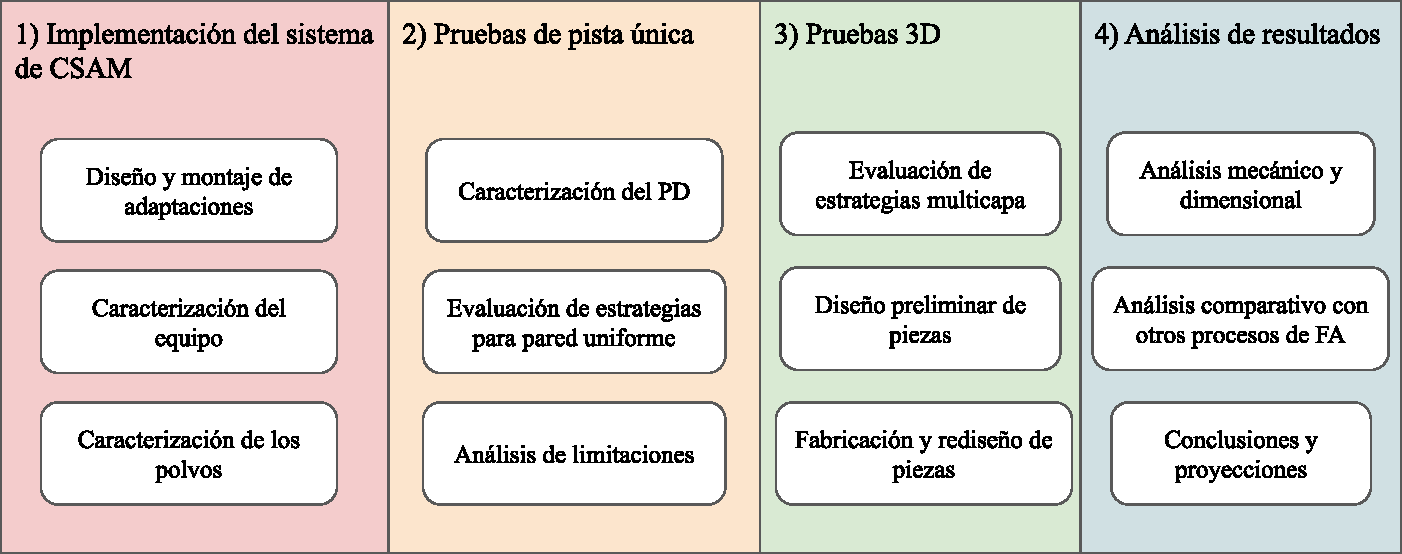
\includegraphics[width=1.0\linewidth]{imgs/etapas.pdf}
	\caption[Flujo de trabajo para el desarrollo de la investigación]{Flujo de trabajo para el desarrollo de la investigación.}
	\label{fig:etapas}
\end{figure}

\section{Implementación de un sistema experimental de CSAM}

\subsection{Recursos}

El desarrollo de este trabajo requirió la implementación de una máquina CNC adaptada para CS, en base al sistema descrito en la sección 2.1.1 y utilizando recursos del grupo de investigación de la Universidad de Chile.

\subsubsection{Arquitectura cinemática}

La arquitectura cinemática utilizada corresponde a una fresadora de escritorio \textit{Pocket NC V2-10} (Figura~\ref{pocket}), cuyas especificaciones relevantes se presentan en el Cuadro~\ref{datospocket}. Esta máquina CNC cuenta con cinco ejes de libertad, lo cual permite proponer estrategias de compensación de paredes mediante variación del ángulo de deposición, tal como se propone en los trabajos de Chepillo et al.~\cite{Chepillo2024} y Wu et al.~\cite{WU2025642}.

\begin{figure}[h!]
	\centering
	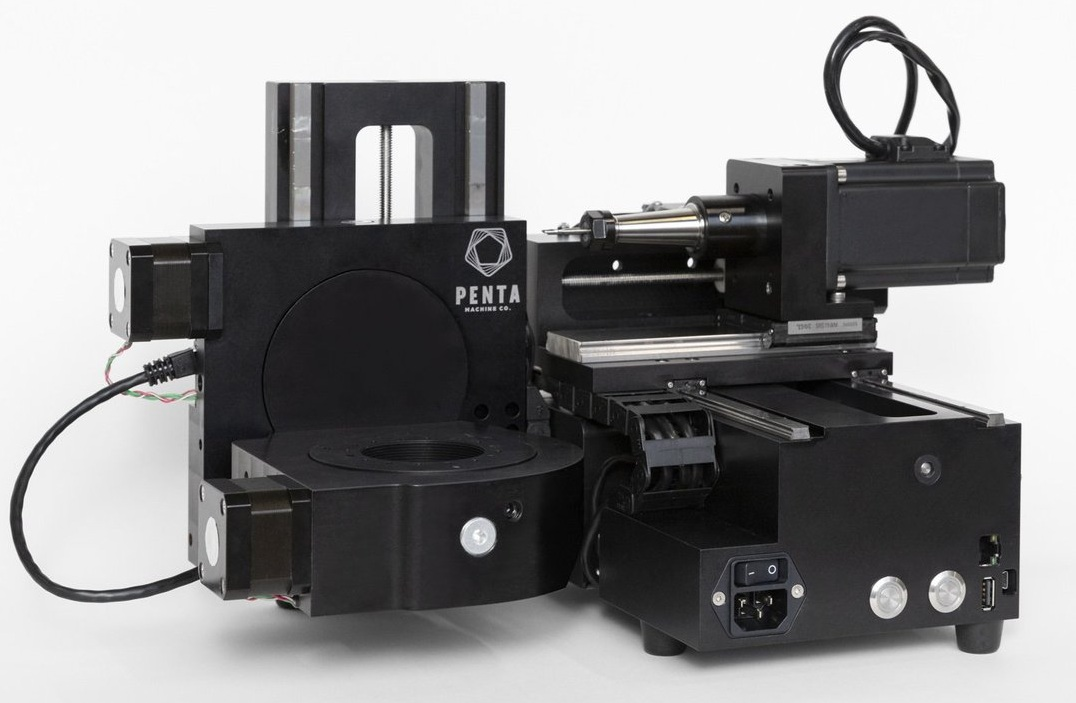
\includegraphics[width=0.6\linewidth]{imgs/pocketnc.jpg}
	\caption[Fresadora de escritorio Pocket NC V2-10]{Fresadora de escritorio Pocket NC V2-10. Fuente: Penta Machine Co}
	\label{pocket}
\end{figure}

\begin{table}[h]
	\centering
	\caption[Especificaciones relevantes de la fre.
	sadora \textit{Pocket NC V2-10}]{Especificaciones relevantes de la fresadora \textit{Pocket NC V2-10. Fuente: Penta Machine Co}.}
	\label{datospocket}
	\begin{tabular}{lccccc}
		\hline
		Parámetro & X & Y & Z & A & B \\
		\hline
		Recorrido     & 115.5 mm & 128.3 mm & 90.1 mm & -25° a 135° & Contínuo \\
		Velocidad max                & 1524 mm/min &  1524 mm/min  &  1524 mm/min & 40 °/s & 40 °/s  \\
		Backlash                         & 12.7 $\mu$m & 12.7 $\mu$m & 12.7 $\mu$m & 0.01° & 0.01° \\
		Resolución                       & 6.1 $\mu$m & 6.1 $\mu$m & 6.1 $\mu$m & 0.01° & 0.01° \\
		Repetibilidad                    & 12.7 $\mu$m & 12.7 $\mu$m & 12.7 $\mu$m & 0.05° & 0.05° \\
		\hline
	\end{tabular}
\end{table}

La conversión de esta máquina para uso en CS requiere dos adaptaciones principales: el reemplazo del husillo de mecanizado por un calefactor de gas, y la protección de los elementos de transmisión frente al flujo de gas caliente y al material particulado que no se adhiere al sustrato.

\subsubsection{Calefactor de gases}

El calefactor de gases es de fabricación propia. Consiste en una estructura tubular de acero inoxidable con dos cámaras concéntricas: el gas ingresa radialmente hacia la cámara 1, y fluye axialmente hasta la entrada de la cámara 2 y luego hasta la salida, donde se conecta con la tobera mediante una rosca NPT 1/4 hembra. En la cámara interior se aloja un calefactor eléctrico tipo barra de 1~kW monofásico con disipadores anulares adosados mediante prisioneros, los cuales además cuentan con perforaciones para el paso del flujo de gas. Esta configuración de doble cámara permite mantener la superficie exterior del calefactor refrigerada, reduciendo el riesgo térmico sobre los componentes cercanos.

\begin{figure}[h!]
	\centering
	\includegraphics[width=0.9\linewidth]{imgs/kalefa.png}
	\caption[Modelo 3D para calefactor de 1kW a) vista isométrica b) vista en corte]{Modelo 3D para calefactor de 1kW}
	\label{fig:kalefa}
\end{figure}

El control de temperatura se implementa mediante un controlador PID digital comercial modelo \textbf{[COMPLETAR: modelo PID]}, que opera a través de un relé de estado sólido. La temperatura de proceso se mide con una termocupla tipo K modelo \textbf{[COMPLETAR: modelo termocupla]}, dispuesta radialmente en la salida del calefactor, aguas arriba de la tobera. De este modo, la variable controlada es la temperatura del gas en la entrada de la tobera, lo cual constituye la temperatura de estancamiento $T_0$ del proceso.

\subsubsection{Gases de proceso}

El gas portador utilizado es nitrógeno (N\textsubscript{2}) con una pureza del \textbf{[COMPLETAR: \%]} por ciento. El suministro se realiza desde dos cilindros de \textbf{[COMPLETAR: volumen]} litros a una presión máxima de \textbf{[COMPLETAR: presión]} bar, cada uno equipado con manómetro y regulador de presión independiente. Los dos cilindros operan en líneas separadas: uno suministra el gas portador principal al calefactor, y el otro alimenta el gas de arrastre del alimentador de polvos. Esta separación permite controlar de forma independiente la presión de proceso y la tasa de inyección de partículas.

El calefactor requiere un pre-calentamiento antes de iniciar la operación de CS, para lo cual se hace circular aire a presión desde un compresor para ahorrar costos. El cambio hacia el gas de proceso se hace manualmente a través de una válvula de 3 posiciones.

\subsubsection{Alimentador de polvos}

El alimentador de polvos utilizado es un modelo PF-SB-2855 de marca \textit{Metallizing Equipment Co}, el cual opera mediante disco rotatorio para regular la tasa de alimentación (Figura \ref{fig:alim}). Este equipo se conecta a uno de los tanques de N2, su presión máxima de operación es de 2.5 bar, cuenta con un rotámetro de hasta 32 SLPM (\textit{standard liter per minute}).

\begin{figure}[h!]
	\centering
	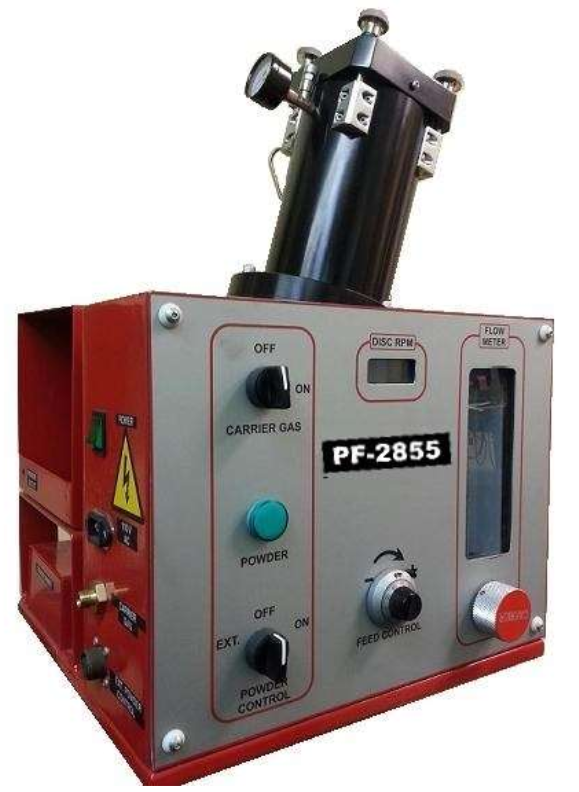
\includegraphics[width=0.3\linewidth]{imgs/alimentador.png}
	\caption[Alimentador de polvo PF-SB-2855]{Alimentador de polvo PF-SB-2855. Fuente: mecpl.com}
	\label{fig:alim}
\end{figure}


\subsubsection{Toberas}

A partir del trabajo de Cerda et al., se fabricaron dos toberas convergente-divergentes de acero inoxidable mediante EDM, cuyos modelos 3D se exhibe en la Figura~\ref{fig:toberas} y cuyas dimensiones principales se presentan en el Cuadro~\ref{tab:geometria_toberas}. Ambas toberas comparten un diámetro de garganta de 1~mm y un diámetro de salida de 3~mm. Se descartó el uso de gargantas de 0{,}5~mm debido al mayor riesgo de obstrucción por partículas, deterioro prematuro por erosión, y sobre-expansión del gas. Las toberas cuentan con una rosca macho NPT 1/4 en uno de sus extremos para la conexión con el calefactor

\begin{figure}[h!]
	\centering
	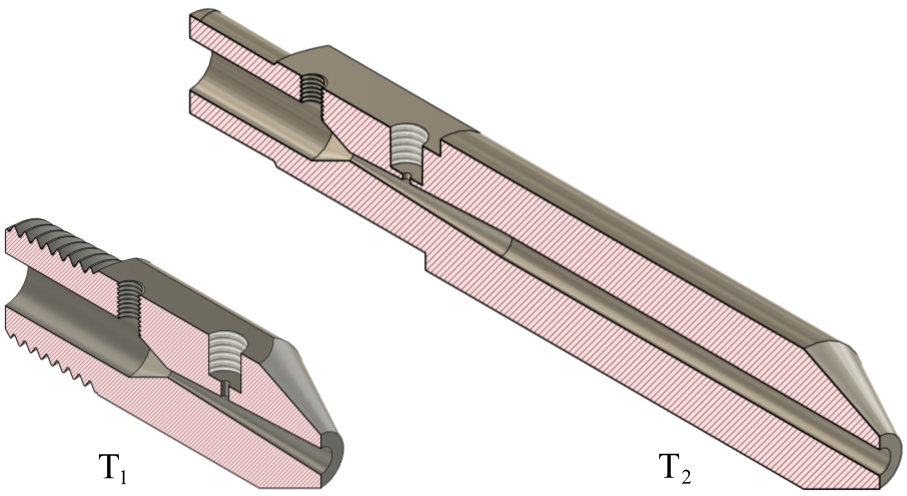
\includegraphics[width=0.7\linewidth]{imgs/toberasblanki.png}
	\caption[Modelos 3D de toberas fabricadas en base a Cerda et al.]{Modelos 3D de toberas fabricadas en base a Cerda et al.}
	\label{fig:toberas}
\end{figure}

Las toberas disponen de una entrada tipo downstream para la inyección de polvo; en caso de que esta configuración no resulte efectiva, se contempla la alternativa de emplear la entrada upstream. La entrada que no se utiliza queda sellada mediante un prisionero y sellante. Adicionalmente, y en caso de que se use la entrada upstream, se plantea conectar una termocupla en la entrada downstream con el fin de obtener una estimación más precisa de la temperatura de remanso $T_{0}$.

La diferencia principal entre las dos toberas radica en la presencia de una sección de barril en la tobera T2: esta extensión downstream de la sección divergente aumenta el tiempo de residencia de las partículas en el jet, favoreciendo la transferencia de momentum y de calor desde el gas hacia las partículas, y permitiendo un mejor desarrollo y estabilización del flujo. En consecuencia, se espera que la tobera con barril produzca mayores velocidades de impacto y temperaturas de partícula. Por otro lado, la sección de barril puede incrementar las pérdidas energéticas por fricción y presentar mayor desgaste por erosión en operación prolongada.La tobera T1, al carecer de barril, presenta una longitud total menor, lo que podría reducir la dispersión radial del jet y disminuir el diámetro efectivo del punto de deposición (\textit{spot}). 

\begin{table}[h]
	\centering
	\caption{Parámetros geométricos de las toberas T1 y T2.}
	\label{tab:geometria_toberas}
	\begin{tabular}{lcc}
	\hline
		\textbf{Parámetro} & \textbf{T1} & \textbf{T2} \\
	\hline
		Diámetro de entrada, $D_{in}$ (mm)         & 6 & 6 \\
		Diámetro de garganta, $D^*$ (mm)           & 1 & 1 \\
		Diámetro de salida, $D_{out}$ (mm)         & 3 & 3 \\
		Largo sección convergente, $L_{conv}$ (mm) & 20 & 20 \\
		Largo sección divergente, $L_{div}$ (mm)   & 20 & 20 \\
		Largo sección de barril, $L_{bar}$ (mm)    & 0 & 50 \\
	\hline
	\end{tabular}
\end{table}

Esta componente es fundamental para definir los parámetros operativos y proyectar las estrategias y resultados obtenibles en el proceso, por lo que se describen en detalle en la sección 3.2.1

\subsection{Adaptaciones mecánicas}

En la Figura~\ref{montfinal} se muestra el modelo 3D de las modificaciones 
realizadas en torno a la máquina CNC para la integración del sistema de CS. 
A continuación se describen cada una de ellas de acuerdo a la numeración en la Figura.

\begin{figure}[h!]
	\centering
	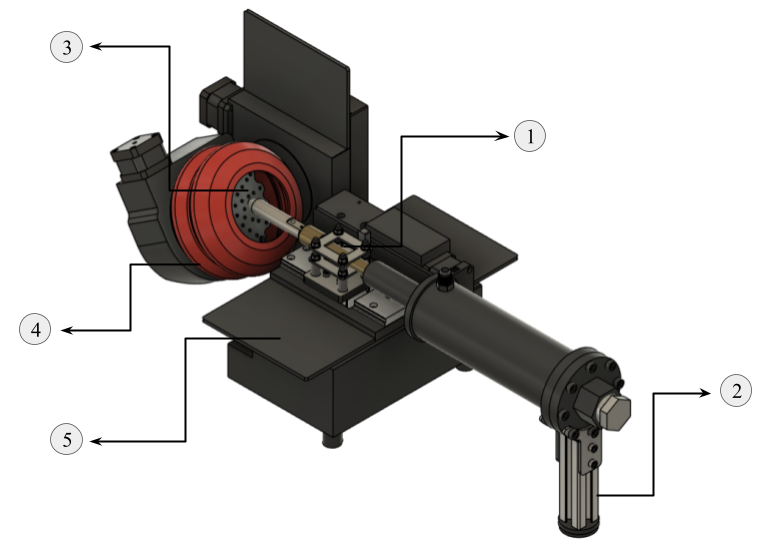
\includegraphics[width=0.75\linewidth]{imgs/3dsys.png}
	\caption[Modelo 3D de las adaptaciones en torno a la máquina CNC ]{Modelo 3D de las adaptaciones en torno a la máquina CNC.}
	\label{montfinal}
\end{figure}

\textbf{1)} En la salida del calefactor se instala una extensión tubular de bronce cuya 
función es aumentar la distancia entre el cuerpo principal del calefactor y 
la estructura de la máquina CNC, reduciendo así los efectos de transferencia 
de calor por radiación. Esta extensión se ancla a la máquina mediante el 
conjunto de soportes mostrado en la Figura~\ref{fig:carro}, sincronizando 
sus movimientos con los ejes $X$ y $Z$. En este mismo conjunto se monta una 
pieza portadora de un imán permanente, cuya función es activar el sensor de 
fin de carrera del eje $Z$ en la posición de referencia.



\textbf{2)} Dado que la masa del calefactor es significativa en relación a la capacidad 
de carga del cabezal de la Pocket NC, se incorporó un apoyo rodante en la 
parte posterior del calefactor. Este consiste en soportes de acero 
inoxidable, un perfil de aluminio de sección T-slot 3030 y un rodamiento 
axial, permitiendo que el calefactor deslice libremente sobre la mesa de 
trabajo sin sobrecargar el cabezal.


\begin{figure}[h!]
	\centering
	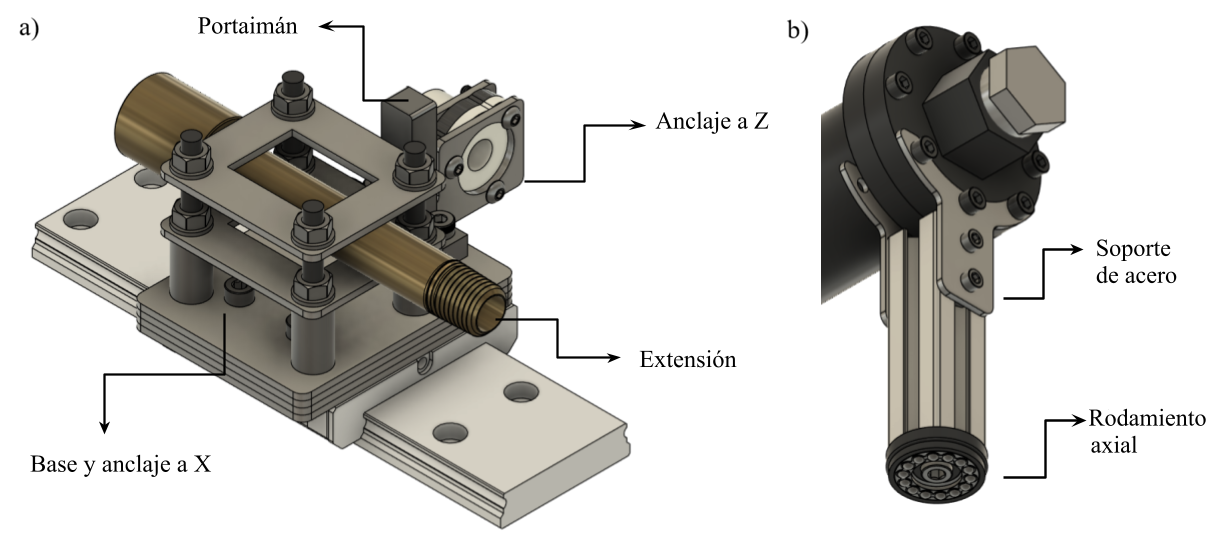
\includegraphics[width=0.9\linewidth]{imgs/parte1.png}
	\caption[Adaptaciones a la máquina CNC, ejes X y Z]{Adaptaciones a la máquina CNC, ejes X y Z. a) Modificación 1: Soporte y anclaje para el calefactor en X y Z, b) Modificación 2: soporte posterior para el calefactor.}
	\label{fig:carro}
\end{figure}

\textbf{3)} Sobre la mesa de trabajo se montan piezas circulares de soporte que cumplen 
dos funciones: fijar el sustrato mediante patrones de apernadura, y canalizar 
el flujo de gas y material particulado no adherido hacia la parte posterior 
del espacio de trabajo, donde es capturado por el sistema de extracción (Figura \ref{fig:parte2}). Los anclajes al eje B de la máquina están espaciados de la base perforada a través de separadores de bronce con rosca.

\textbf{4)}Para confinar el flujo de gases y polvo, el espacio de trabajo se encierra 
mediante un fuelle de silicona fabricado a medida. El material empleado es 
silicona de alta temperatura (hasta \SI{290}{\celsius}) de la marca 
Smooth-On, la cual combina resistencia térmica con alta elasticidad, 
permitiendo el desplazamiento libre de la tobera sobre el sustrato sin 
comprometer el sellado del espacio.

\begin{figure}[h!]
	\centering
	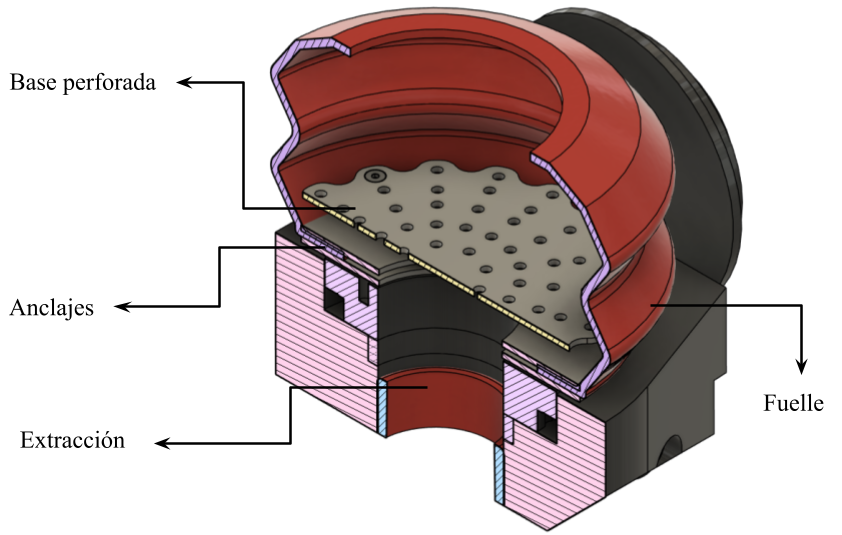
\includegraphics[width=0.8\linewidth]{imgs/parte2.png}
	\caption[Vista en corte de las adaptaciones en el espacio de trabajo]{Vista en corte de las adaptaciones en el espacio de trabajo.}
	\label{fig:parte2}
\end{figure}

\textbf{5)} Finalmente, los rieles lineales de la máquina CNC se protegen mediante 
placas de aluminio compuesto fijadas a las partes móviles de la máquina, 
previniendo el desgaste por polvo sobre los mecanismos 
de guía.

\subsection{Sistema de extracción}

El dimensionamiento del sistema de extracción se realizó considerando el caudal del jet de gases a la salida de la tobera y el aire ambiente arrastrado por el jet libre. El caudal del jet $Q_0$ se estimó considerando una velocidad promedio de referencia de $\bar{v} = 1000$~m/s en la sección de salida de la tobera de diámetro $d_s = 3$~mm, de acuerdo a las simulaciones de Cerda et al.:

\begin{equation}
	Q_0 = \frac{\pi d_s^2}{4} \cdot \bar{v} = \frac{\pi (0{,}003)^2}{4} \cdot 1000 \approx 7{,}07 \times 10^{-3}~\text{m}^3/\text{s}
	\label{eq:qjet}
\end{equation}

El caudal total del jet a una distancia axial $x$ de la salida, incluyendo el aire ambiente arrastrado, se estima mediante la correlación de Ricou y Spalding~\cite{RicouSpalding1961} para jets turbulentos libres axisimétricos:

\begin{equation}
	\frac{Q(x)}{Q_0} = 0{,}32 \cdot \frac{x}{d_s} \cdot \left(\frac{\rho_0}{\rho_\infty}\right)^{1/2}
	\label{eq:entrainment}
\end{equation}

donde $\rho_0$ es la densidad del gas en la sección de salida y $\rho_\infty$ es la densidad del aire ambiente. De acuerdo con las simulaciones de Cerda et al., la temperatura del gas a la salida de la tobera se sitúa en torno a 200–250~°C, correspondiente a aproximadamente 500~K. A esa temperatura y a presión atmosférica, la densidad del N$_2$ es $\rho_0 \approx 0{,}67$~kg/m$^3$, mientras que para el aire ambiente a 20~°C se tiene $\rho_\infty \approx 1{,}20$~kg/m$^3$. Tomando como distancia de referencia $x = 100$~mm, correspondiente a la distancia aproximada entre la salida de la tobera y la pared del fuelle:

\begin{equation}
	\frac{Q(x)}{Q_0} = 0{,}32 \cdot \frac{0{,}1}{0{,}003} \cdot \left(\frac{0{,}67}{1{,}20}\right)^{1/2} \approx 0{,}32 \cdot 33{,}3 \cdot 0{,}747 \approx 7{,}96
	\label{eq:ratio_entrainment}
\end{equation}

El caudal total que debe manejar el sistema de extracción resulta entonces:

\begin{equation}
	Q_\text{total} = 7{,}96 \cdot Q_0 \approx 7{,}96 \times 7{,}07 \times 10^{-3} \approx 5{,}63 \times 10^{-2}~\text{m}^3/\text{s} \approx 56{,}3~\text{L/s}
	\label{eq:qtotal}
\end{equation}

Cabe destacar que esta estimación corresponde a un jet libre no confinado, por lo que representa un escenario conservador: en la práctica, el fuelle limita el volumen de aire disponible para el entrainment, reduciendo el caudal efectivo. Aplicando un factor de seguridad de 1{,}5 sobre el caudal estimado, se requiere una aspiradora con una capacidad mínima de aproximadamente 85~L/s (305~m$^3$/h). Con base en este análisis, se seleccionó una aspiradora industrial modelo HT-60 de marca Luster con un caudal nominal de 106 L/s, contenedor de acero inoxidable y compatible con filtro HEPA.

\subsection{Material pulverizado y sustrato}

El material utilizado para los depósitos corresponde a polvo de titanio
comercialmente puro Grado~4 (CP-Ti Gr.~4) Metco 4010 de Oerlikon, fabricado mediante el proceso
de hidruración-deshidruración (HDH) a partir de materia prima forjada,
lo cual confiere a las partículas una morfología poliédrica irregular, con facetas planas bien definidas (\textit{blocky}) (Figura \ref{polvi}). Las principales características del polvo, según la
hoja de datos del proveedor~\cite{Metco4010}, se resumen en la
Tabla~\ref{tab:polvo_cpti}.

\begin{figure}[h!]
	\centering
	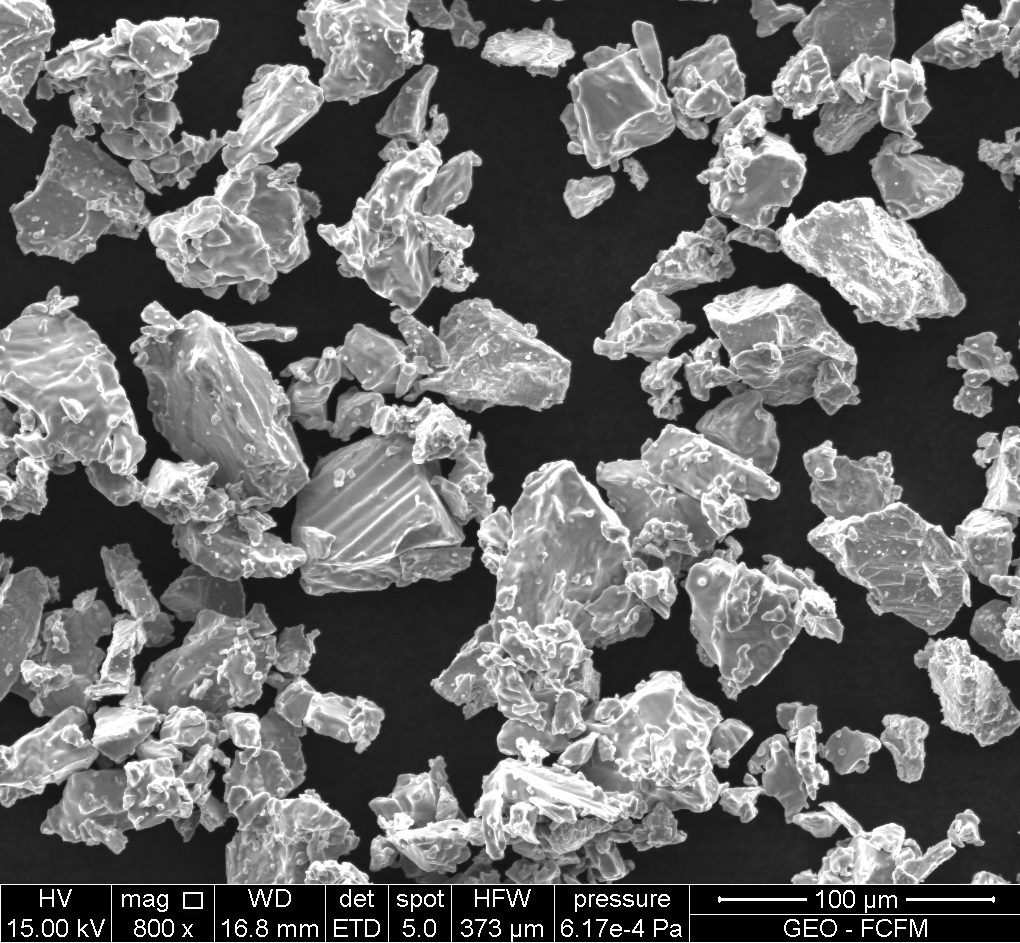
\includegraphics[width=0.7\linewidth]{imgs/bloki.png}
	\caption{Imagen obtenida por microscopía (SEM) del polvo 4010 C. }
	\label{polvi}
\end{figure}

\begin{table}[h]
	\centering
	\caption[Características del polvo CP-Ti Grado~4 empleado]{Características del polvo CP-Ti Grado~4 empleado
		(Oerlikon Metco, serie Metco~4010~\cite{Metco4010}).}
	\label{tab:polvo_cpti}
	\begin{tabular}{ll}
		\hline
		\textbf{Parámetro} & \textbf{Valor} \\
		\hline
		Función primaria & Biocompatibilidad \\
		Composición nominal & Ti Grado~4 (ASTM) \\
		Proceso de fabricación & HDH a partir de material forjado \\
		Morfología & Angular (\textit{blocky}) \\
		Distribución granulométrica & $-45{+}11~\mu$m \\
		Temperatura de fusión & \SI{1649}{\celsius} \\
		Fe máx. (wt\%) & 0{,}50 \\
		O máx. (wt\%) & 0{,}40 \\
		C máx. (wt\%) & 0{,}08 \\
		N máx. (wt\%) & 0{,}05 \\
		H máx. (wt\%) & 0{,}015 \\
		\hline
	\end{tabular}
\end{table}

Para estos experimentos, el sustrato constituye un elemento de sacrificio:
el objetivo es obtener la pieza depositada, por lo que el criterio de
selección prioriza la facilidad de adhesión por sobre cualquier otra
consideración funcional.

El sustrato elegido corresponde a aluminio 1100, suministrado en formato
de plancha de 5~mm de espesor, cortado mediante sierra y CNC en las
geometrías requeridas por cada experimento. Este material fue seleccionado
por su amplia disponibilidad comercial y por constituir un sustrato de
referencia habitual en experimentos de CS, gracias a su bajo límite de
fluencia y elevada plasticidad \cite{Yin2014substrate}.

Su microestructura es esencialmente monofásica ---fase $\alpha$-Al con
escasa presencia de precipitados--- lo que le confiere una respuesta
plástica homogénea y un endurecimiento por deformación progresivo bajo
impacto a alta velocidad. Esta combinación favorece el colapso superficial
continuo y el anclaje mecánico por incrustación de las partículas de Ti,
promoviendo el contacto íntimo metal--metal necesario para la adhesión
\cite{Binder2011}. La asimetría de dureza entre el Ti proyectado
($\sim$150--180~HV) y el sustrato de Al ($\sim$30--50~HV)
\cite{Callister2018} concentra la deformación plástica en el sustrato,
condición que, como se discutió en la sección anterior, es favorable para
la deposición.

Respecto a la capa de óxido nativo ---principalmente
Al\textsubscript{2}O\textsubscript{3}, de alta dureza y estabilidad
química--- su presencia no constituye una limitación crítica, ya que
durante el impacto la deformación plástica intensa en el metal subyacente
induce la fractura y dispersión del óxido, permitiendo el contacto
metal--metal necesario para la formación del enlace \cite{Assadi2003}.
Asimismo, dado que la escala de tiempo del impacto es varios órdenes de
magnitud inferior a la escala de difusión térmica, la elevada conductividad
del aluminio 1100 no interviene en la dinámica interfacial adiabática; su
efecto se limita a favorecer una distribución homogénea del calor durante
el precalentamiento previo al proceso, contribuyendo a la estabilidad
de las condiciones superficiales.

\subsection{Sistema final}

El diagrama del sistema final se observa en la Figura \ref{esqumesis}. El eje A de la máquina debe posicionarse por defecto a 90° respecto a su referencia, de modo que el sustrato quede orientado normal al eje de la tobera. La máquina CNC se conecta mediante USB a un computador, a través del cual se carga y ejecuta el código G generado para cada trayectoria. 

\begin{figure}[h!]
	\centering
	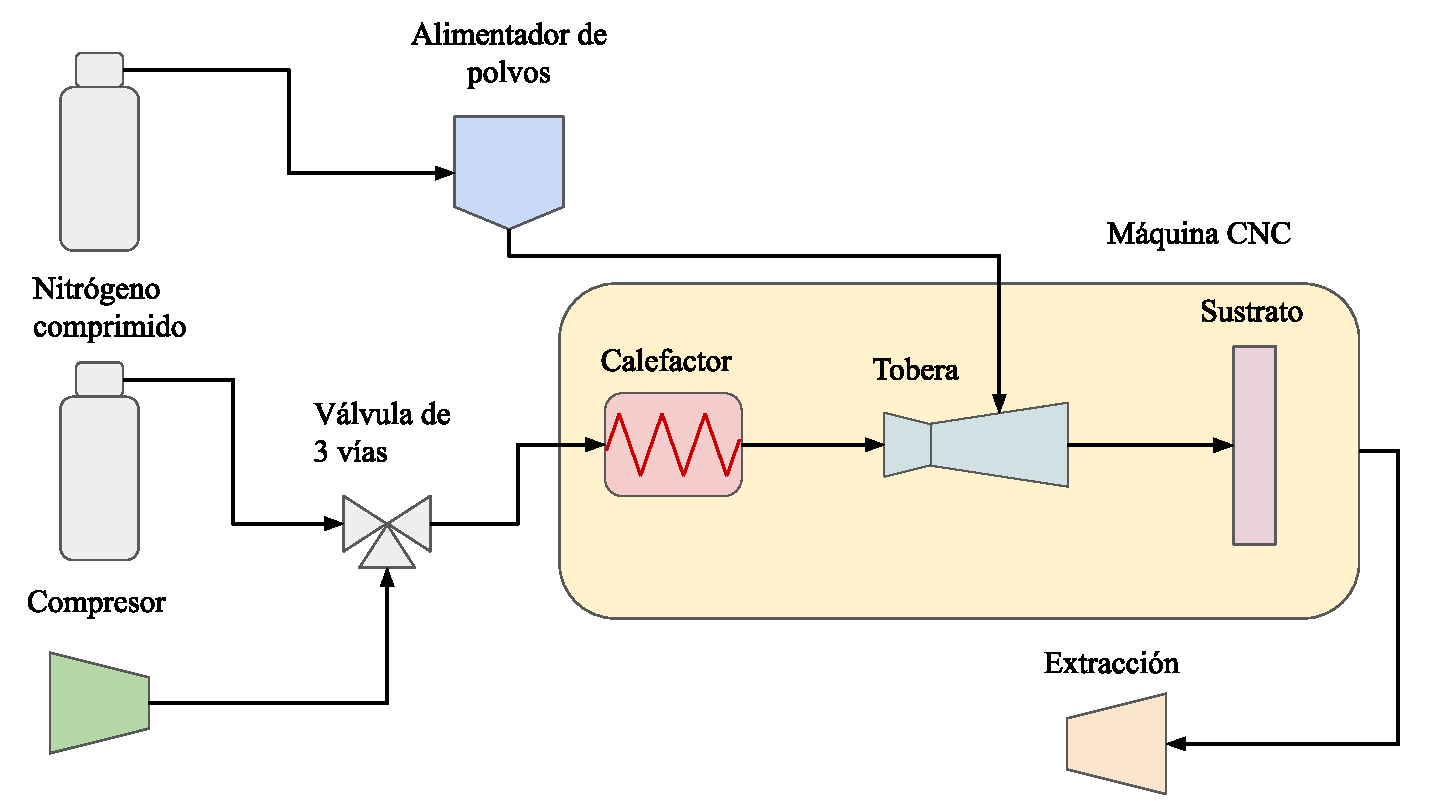
\includegraphics[width=0.9\linewidth]{imgs/diagsys.pdf}
	\caption{Diagrama del sistema de CS implementado.}
	\label{esqumesis}
\end{figure}


Este código G se escribe a través de programas específicos implementados en Python para cada experimento y estrategia o pieza a lograr, pues no se cuenta con un software CAM para el proceso.

La máquina no dispone de un sistema de deflexión o bloqueo del jet, por lo que no es posible detener la proyección de partículas en los movimientos sin fabricar de las trayectorias, o durante la preparación del jet antes de fabricar.

\subsection{Caracterización del espacio de trabajo}

Con el sistema ensamblado se realizaron pruebas de movimiento para determinar el espacio de trabajo útil respecto a las capacidades nominales de la máquina original. Posicionando la tobera en contacto con la periferia del área de trabajo y recorriendo su contorno, se comprueba que es posible recorrer la circunferencia completa deformando ligeramente la protección de silicona. En consecuencia, el espacio de trabajo útil puede definirse en coordenadas cilíndricas según el Cuadro~\ref{tab:espacio_trabajo} para la configuración estándar de la máquina con el eje A a 90°.

\begin{table}[h]
	\centering
	\caption{Espacio de trabajo útil del sistema en coordenadas cilíndricas.}
	\label{tab:espacio_trabajo}
	\begin{tabular}{ccc}
		\hline
		Parámetro & Mínimo & Máximo \\
		\hline
		$r$ [mm]      & 0   & \textbf{[COMPLETAR]} \\
		$\theta$ [°]  & 0   & 360 \\
		$z$ [mm]      & 0   & \textbf{[COMPLETAR]} \\
		\hline
	\end{tabular}
\end{table}

Este rango se ve reducido al utilizar el eje A, puesto que la deformación impuesta sobre la protección de silicona aumenta con la desviación angular respecto a la normal, con la profundidad en $z$ y con la desviación radial respecto al centro del área de trabajo, tal como se ilustra en la Figura~\ref{fig:espacio_A}. Dado que la literatura reporta un ángulo crítico de deposición para titanio por encima del cual la eficiencia cae drásticamente~\cite{WU2025642}, se fija el rango operativo del eje A en un mínimo de 70° respecto a la superficie del sustrato. 

\begin{figure}[h!]
	\centering
	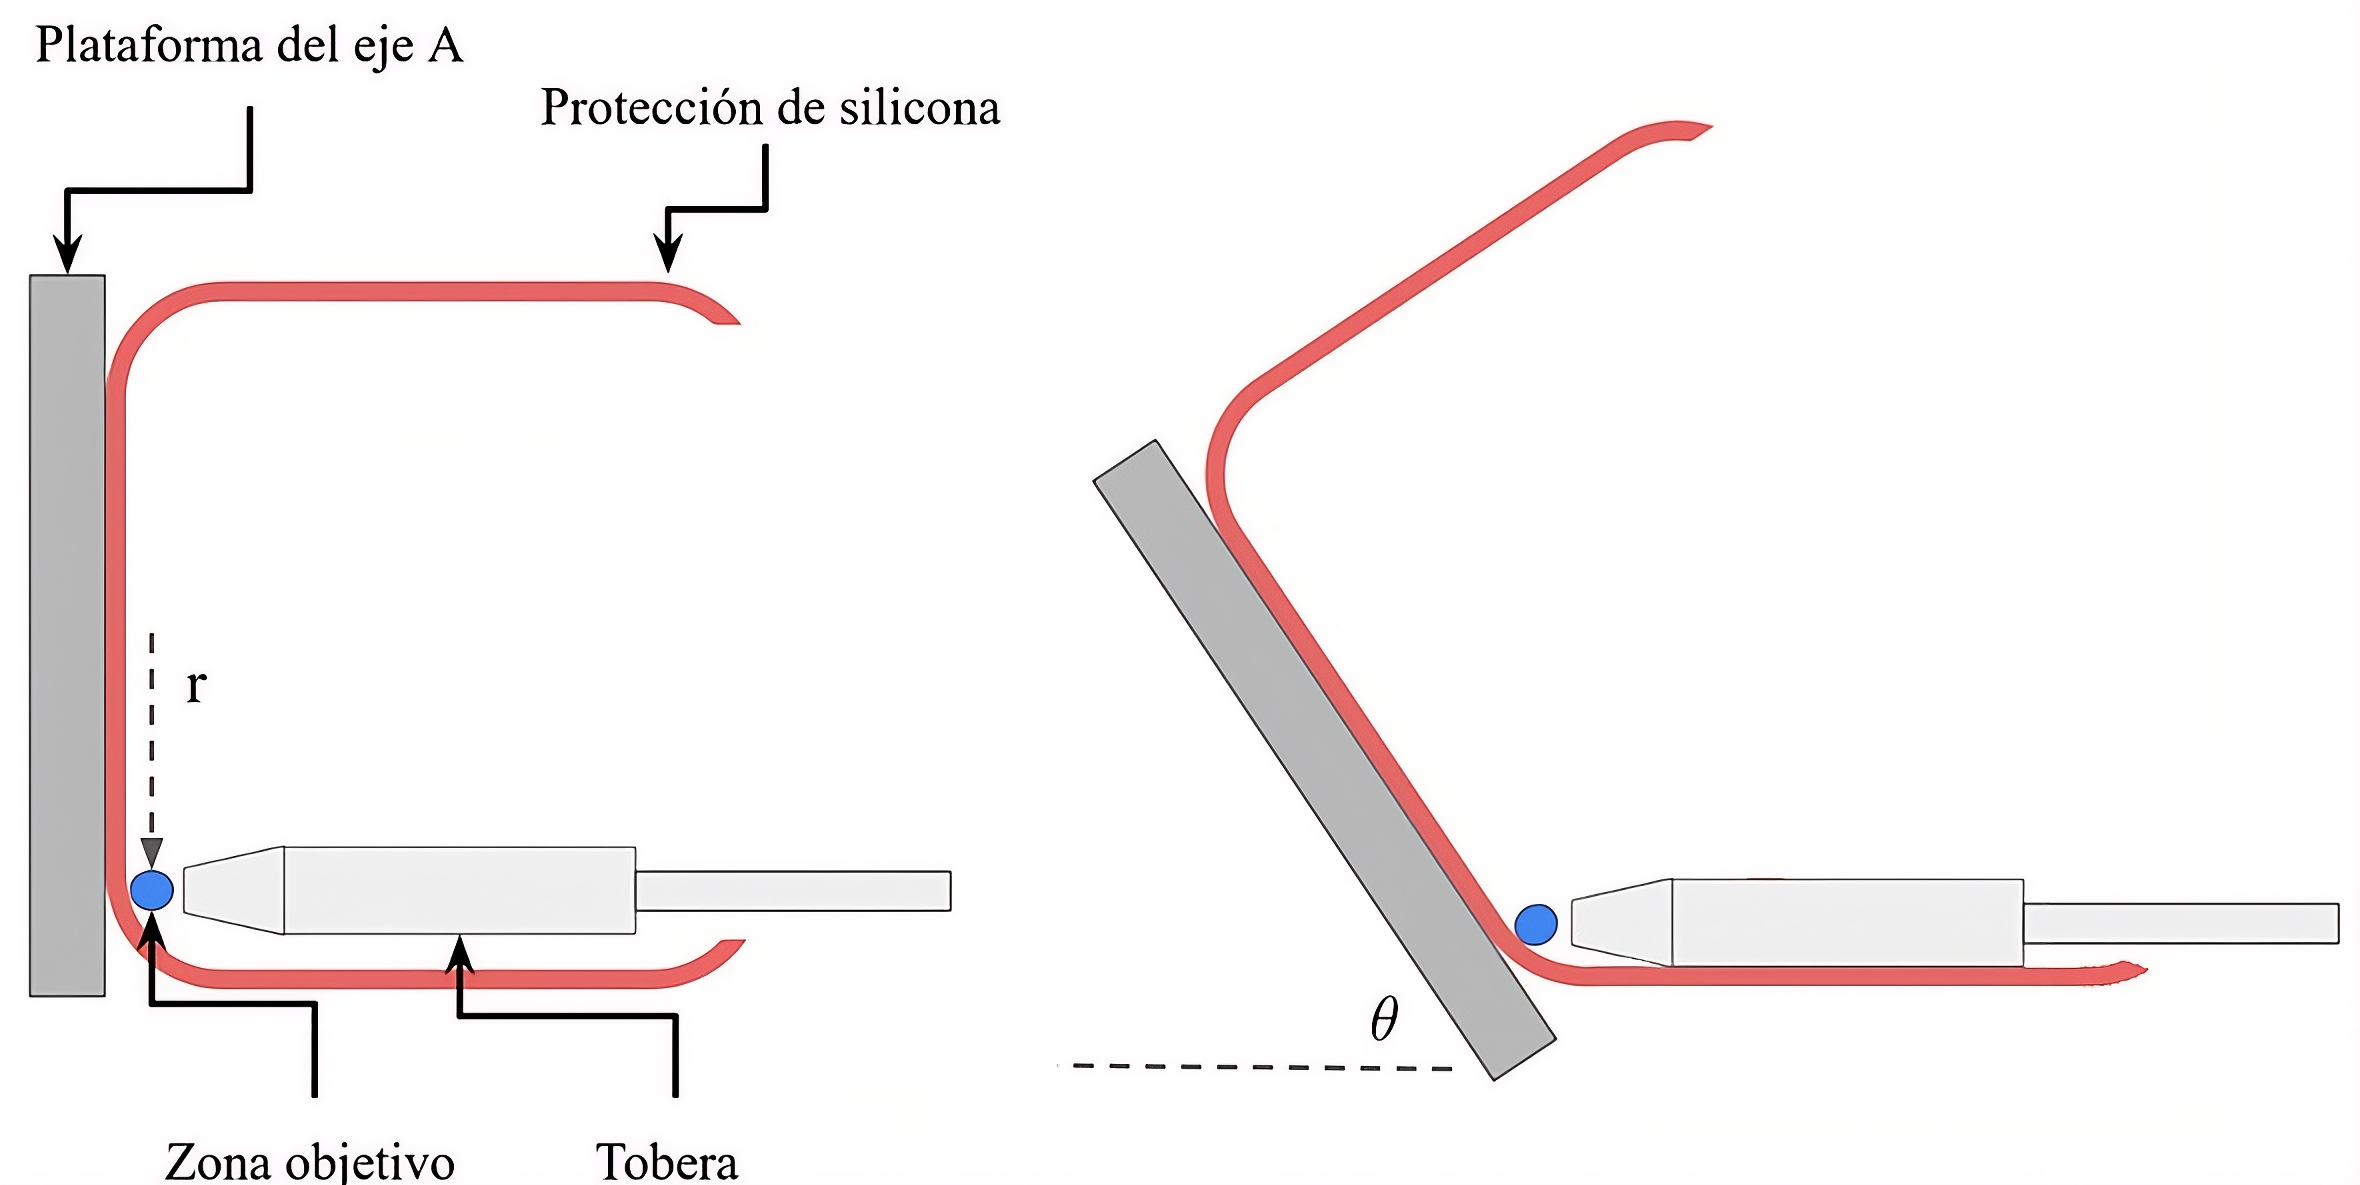
\includegraphics[width=0.9\linewidth]{imgs/anguli.png}
	\caption{Diagrama para la limitación del ángulo de deposición.}
	\label{fig:espacio_A}
\end{figure}

Es importante notar que en fabricación aditiva tridimensional se generan nuevas superficies al construir las paredes que definen un objeto. En un sistema cartesiano convencional, la deposición ocurre siempre sobre la cara superior de la pared en construcción, siguiendo un paradigma de fabricación estrictamente planar. Sin embargo, un sistema con mayor número de grados de libertad ofrece capacidades adicionales: permite depositar de manera oblicua o normal a las caras laterales de las paredes ya fabricadas (Figura~\ref{fig:deposicion_oblicua}), eliminando la necesidad de soportes. En este caso, el ángulo crítico se evalúa respecto a la cara lateral de la pared, lo cual resulta más favorable geométricamente que respecto a la cara superior. Este modo de deposición queda fuera del alcance de la presente investigación, ya que la protección de silicona restringe el acceso lateral a las paredes fabricadas.

\begin{figure}[h!]
	\centering
	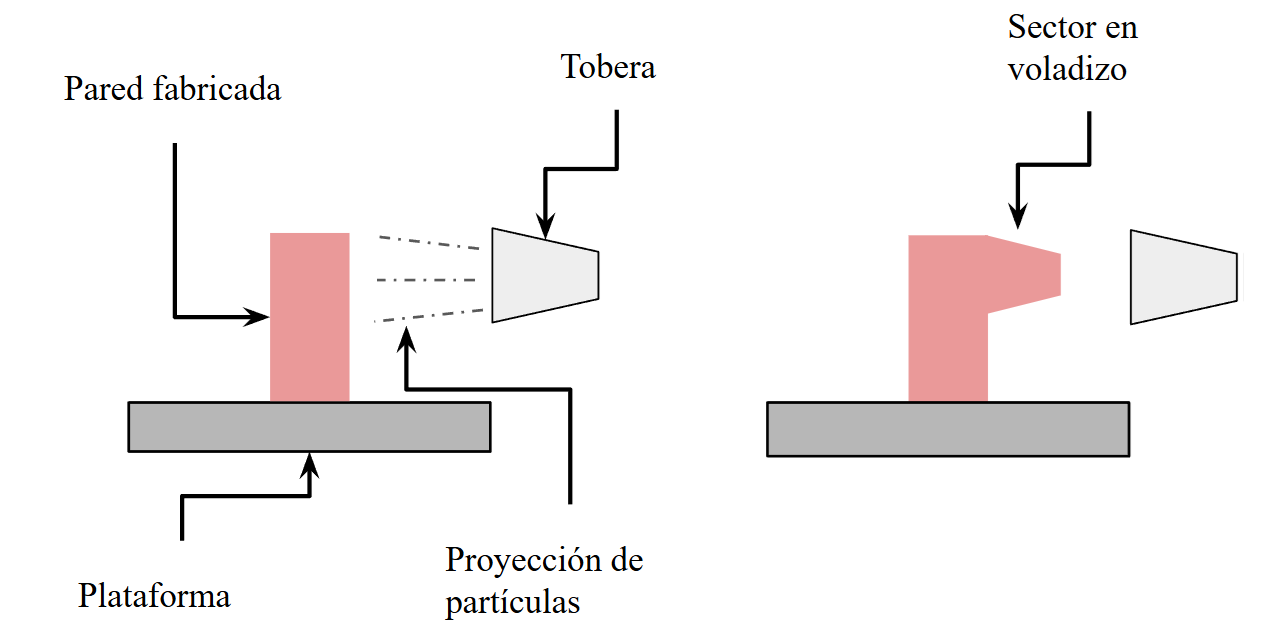
\includegraphics[width=0.8\linewidth]{imgs/volad.png}
	\caption{Generación de sector en voladizo mediante trayectoria no planar.}
	\label{fig:deposicion_oblicua}
\end{figure}


Se reconoce que la protección de silicona constituye un mecanismo sencillo para otorgar contención al proceso; sin embargo, limita la versatilidad de las estrategias y trayectorias de deposición posibles. Una alternativa a esta solución consistiría en construir un recinto rígido y translúcido que cubra la totalidad de la máquina —por ejemplo, una caja de acrílico o policarbonato— equipado con un sistema de extracción de polvo, complementado con cubiertas localizadas sobre las zonas críticas de la máquina, tales como rieles lineales y sectores con movimiento relativo. Una opción adicional sería la incorporación de cortinas de aire dirigidas hacia las superficies a proteger, desviando el polvo suspendido antes de que pueda contaminarlas.

Dado que no es factible la deposición completamente normal a las caras laterales de las paredes fabricadas ni la generación de soportes funcionales, se plantea que un voladizo limitado podría generarse mediante una deposición oblicua ejecutada sobre el borde de una pared ya consolidada o sobrecompensando una pared en fabricación, de modo que el material depositado sobresalga lateralmente, como se observa en la Figura \ref{fig:sopob}

\begin{figure}[h!]
	\centering
	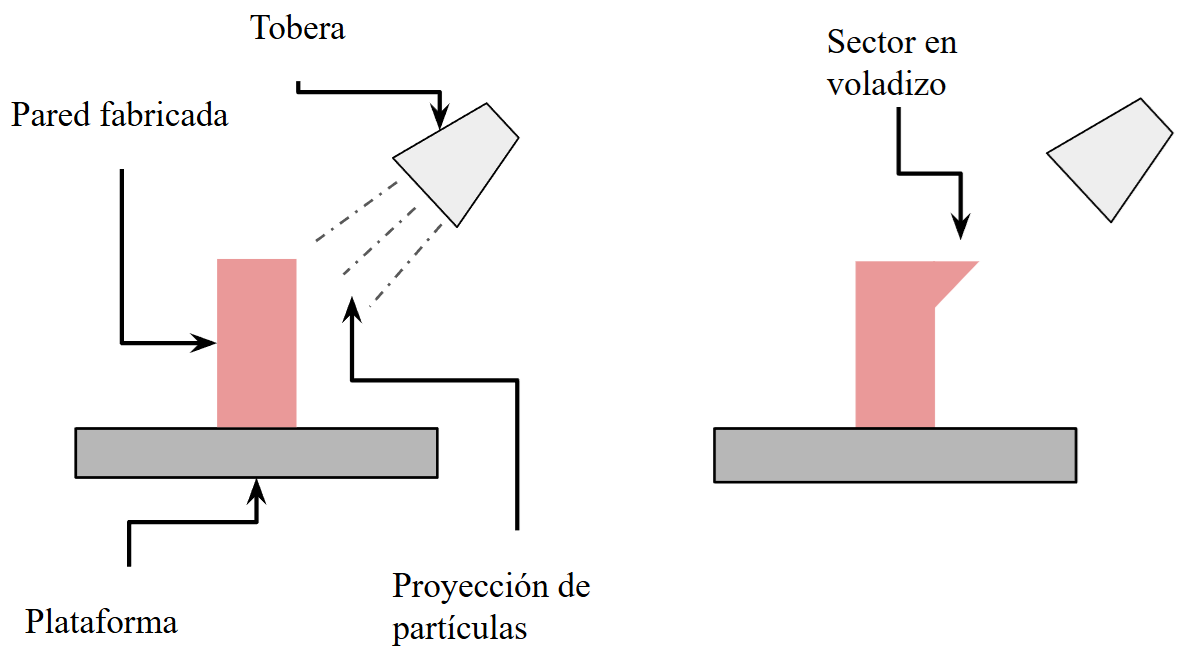
\includegraphics[width=0.8\linewidth]{imgs/volobl.png}
	\caption{Generación de sector en voladizo mediante deposición oblicua.}
	\label{fig:sopob}
\end{figure}

La velocidad máxima de cada eje se verifica con el sistema completamente ensamblado, incluyendo todas las conexiones de polvo, gases y alimentación eléctrica. Durante estas pruebas no se detecta pérdida de pasos ni se registra el sonido característico de desincronización en ninguno de los ejes. Dado que el control de los motores paso a paso de la Pocket NC opera en lazo abierto —sin retroalimentación de posición— la ausencia de estos indicadores constituye el criterio de validación disponible, por lo que se estima que las velocidades máximas nominales se mantienen bajo las condiciones de carga impuestas.

\subsection{Resumen de parámetros operativos}

En el Cuadro~\ref{tab:parametros} se presentan los acrónimos y rangos operativos de los parámetros que gobiernan el proceso en el sistema implementado.

\begin{table}[h]
	\centering
	\caption{Parámetros operativos del sistema de CS implementado y sus rangos de operación.}
	\label{tab:parametros}
	\begin{tabular}{clcc}
		\hline
		Símbolo & Parámetro & Mínimo & Máximo \\
		\hline
		$T_0$       & Temperatura de estancamiento [°C]   & 25 & 480 \\
		$p_0$       & Presión de estancamiento [bar]      & 10   & 20   \\
		$\theta$    & Ángulo de deposición [°]            & 70  & 90  \\
		$v_f$       & Velocidad de avance [mm/min]          & 0 & 1524 \\
		$d_s$       & Distancia de standoff [mm]          & 0 & 50 \\
		\hline
	\end{tabular}
\end{table}

\section{Planificación de experimentos de una capa}

\subsection{Características de las toberas}

Los perfiles de depósito obtenidos experimentalmente están directamente condicionados por las características geométricas y fluidodinámicas de las toberas empleadas. Por ello, antes de planificar los experimentos de pista única, corresponde describir estas toberas y contrastar su desempeño nominal de diseño con el comportamiento real a medir, a modo de establecer el marco de referencia dentro del cual se interpretan los resultados experimentales posteriores.

Las toberas fabricadas fueron simuladas numéricamente en Cerda et al., las
condiciones iniciales se muestran en el Cuadro~\ref{tab:condiciones_cerda}. Los resultados
principales de estas simulaciones se resumen en el Cuadro~\ref{tab:resultados_toberas},
e incluyen la velocidad y temperatura de impacto de la partícula con mayor velocidad para cada
diseño de tobera seleccionado.

\begin{table}[h]
	\centering
	\caption{Condiciones iniciales empleadas en las simulaciones 
		fluido-dinámicas de Cerda et al.}
	\label{tab:condiciones_cerda}
	\begin{tabular}{lc}
		\hline
		\textbf{Parámetro} & \textbf{Valor} \\
		\hline
		Presión de entrada $p_0$       & \SI{3.40}{MPa}       \\
		Temperatura de entrada $T_0$   & \SI{750}{K}          \\
		Presión de salida              & \SI{101.3}{kPa}      \\
		Temperatura de salida          & \SI{300}{K}          \\
		Rango granulométrico $d_p$     & 10--50~$\mu$m        \\
		Morfología del polvo           & Esférica             \\
		Material del polvo             & Ti~CP                \\
		Gas de proceso & $N_{2}$ \\
		\hline
	\end{tabular}
\end{table}

\begin{table}[ht]
	\centering
	\caption{Principales resultados de simulación para las toberas T1 y T2 en Cerda et al.}
	\label{tab:resultados_toberas}
	\begin{tabular}{lcc}
		\hline
		\textbf{Parámetro} & \textbf{T1} & \textbf{T2} \\
		\hline
		Velocidad del gas a la salida (m/s)     & 1076 & 1037 \\
		Velocidad crítica de partícula (m/s)    &  509 &  515 \\
		Velocidad de partícula a la salida (m/s)&  384 &  539 \\
		Temperatura de partícula a la salida (K)&  352 &  320 \\
		Eficiencia de deposición (\%)           &    0 &   28 \\
		\hline
	\end{tabular}
\end{table}

Nótese que en $T_{1}$, a pesar de que el gas alcanza una mayor velocidad de salida
respecto a $T_{2}$, las partículas no logran alcanzar la velocidad crítica teórica
calculada mediante la ecuación~\ref{vcrit}. Este resultado puede atribuirse a la
insuficiente longitud de la sección divergente y, por tanto, al reducido tiempo de
residencia disponible para que las partículas aceleren y sigan la trayectoria del gas
de manera efectiva. Así, la sección de barril en $T_{2}$ otorga más tiempo de residencia y estabiliza el 
flujo, logrando generar deposición, aunque escasa. En la Figura \ref{fig:perfiltobs} se observan los perfiles de deposición simulados durante 1 segundo en posición estática en Cerda et al. para distintas toberas, el perfil para la tobera $T_{2}$ se observa en azul.

\begin{figure}[h!]
	\centering
	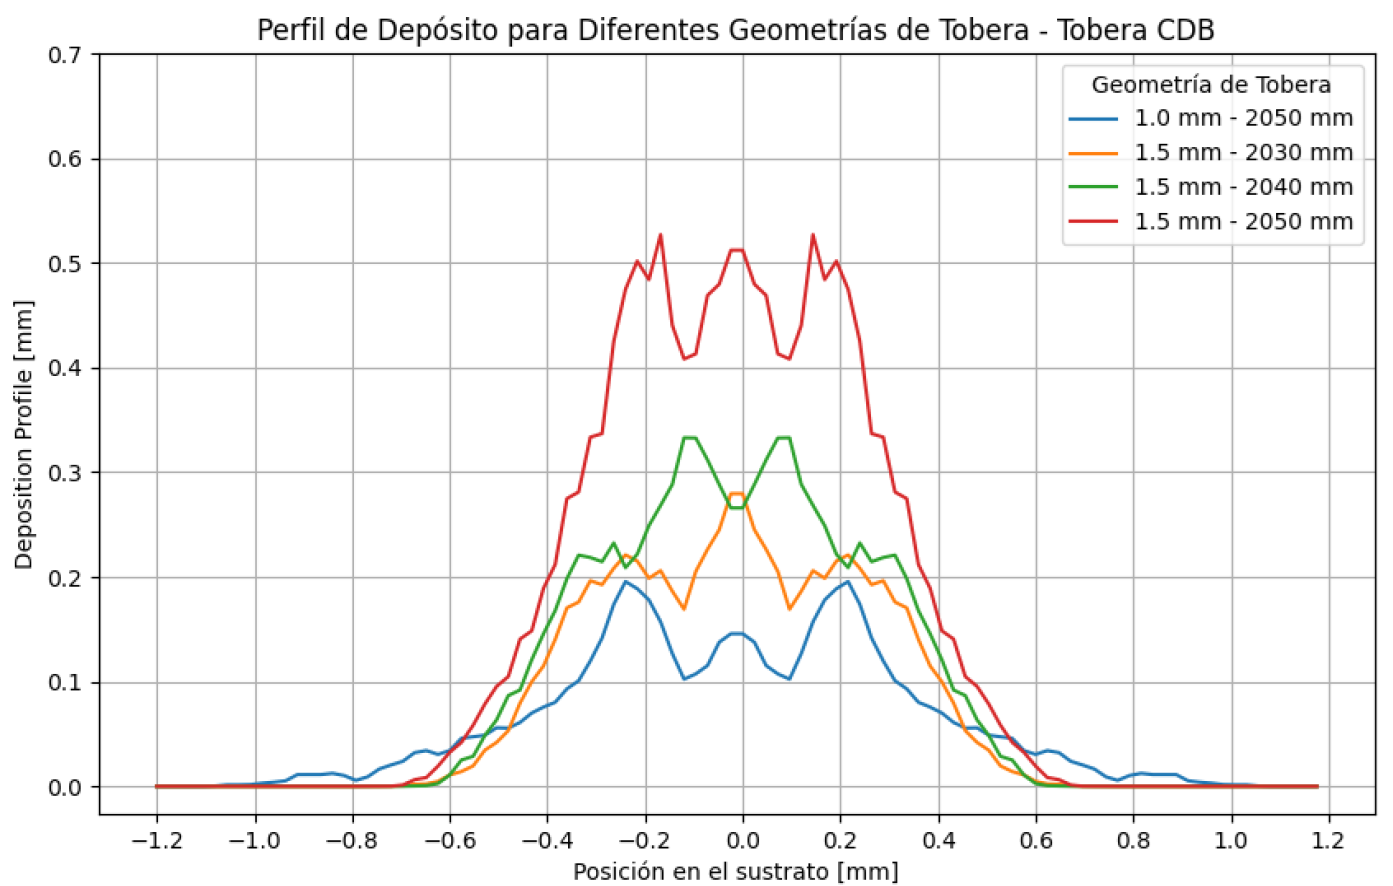
\includegraphics[width=0.8\linewidth]{imgs/perfiltob.png}
	\caption[Perfil de deposición para las toberas efectivas en Cerda et al.]{Perfil de deposición para las toberas efectivas en Cerda et al. \cite{CerdaLobos2024}.}
	\label{fig:perfiltobs}
\end{figure}

Una diferencia relevante entre las simulaciones de Cerda et al. y las 
condiciones experimentales de la presente investigación radica en la 
morfología del polvo: las simulaciones asumen partículas esféricas, 
mientras que el polvo Oerlikon Metco serie 4010 empleado aquí presenta 
morfología irregular de tipo HDH (\textit{blocky}). Esta distinción 
afecta principalmente al coeficiente de arrastre $C_D$, que para 
partículas no esféricas es mayor que el correspondiente a una esfera 
del mismo diámetro equivalente, lo que implica una aceleración 
ligeramente superior bajo las mismas condiciones de gas~\cite{Yin2022review}. 
Por tanto, las velocidades de impacto reportadas por Cerda et al. 
constituyen una estimación conservadora para el polvo HDH empleado, y 
los perfiles de temperatura de partícula permanecen cualitativamente 
válidos dado que el número de Biot se mantiene pequeño en ambos casos.

Un factor crítico que no fue abordado directamente en el estudio de Cerda et al.\ es el análisis 
de la longitud crítica de Fanno, descrita en la sección 2.1.2. Este parámetro 
representa la longitud máxima de ducto de sección constante a partir de la cual un flujo 
supersónico con fricción alcanzaría condiciones sónicas, y su evaluación permite 
cuantificar el efecto de la fricción viscosa sobre el flujo en la sección de barril de 
la tobera.

Para la tobera $T_{2}$, cuya sección de barril posee diámetro $D = \SI{6}{mm}$ y longitud 
$L = \SI{50}{mm}$, se emplearon las condiciones del gas a la entrada de dicha sección, 
estimadas a partir de los resultados de simulación (Figuras \ref{fig:velocipi} y \ref{fig:temp_gas}): velocidad $v_1 \approx \SI{1100}{m/s}$ 
y temperatura $T_1 \approx \SI{200}{K}$. El número de Mach de entrada se calcula como:

\begin{equation}
	M_1 = \frac{v_1}{\sqrt{\gamma R T_1}} = \frac{1100}{\sqrt{1.4 \times 296.8 \times 200}} 
	\approx 3.82
	\label{eq:mach_barril_T2}
\end{equation}

Para el factor de fricción, se consideró la rugosidad superficial característica del 
acero inoxidable mecanizado por EDM, $\varepsilon \approx \SI{1.6}{\micro m}$, lo que 
para $D = \SI{6}{mm}$ entrega una rugosidad relativa $\varepsilon/D \approx 2.67\times10^{-4}$. 
En el régimen de flujo completamente rugoso, la correlación de Colebrook-White simplificada 
entrega \cite{White2016}:

\begin{equation}
	\frac{1}{\sqrt{f}} = -2\log\left(\frac{\varepsilon/D}{3.7}\right) 
	= -2\log(7.21\times10^{-5}) \approx 8.28 
	\implies f \approx 0.0146
	\label{eq:factor_friccion}
\end{equation}

Evaluando la ecuación de Fanno~\eqref{eq:fanno} en $M_1 = 3.82$:

\begin{equation}
	\left.\frac{4fL^{*}}{D}\right|_{M_1} = \frac{1-M_1^2}{\gamma M_1^2} + 
	\frac{\gamma+1}{2\gamma}\ln\left(\frac{(\gamma+1)M_1^2}{2\left(1+
		\dfrac{\gamma-1}{2}M_1^2\right)}\right) \approx 0.618
	\label{eq:fanno_eval}
\end{equation}

de donde se obtiene la longitud crítica:

\begin{equation}
	L^{*}_{T_{2}} = \frac{0.618 \times D}{4f} = 
	\frac{0.618 \times \SI{6}{mm}}{4 \times 0.0146} \approx \SI{63.5}{mm}
	\label{eq:fanno_T2}
\end{equation}

Dado que la sección de barril mide $L = \SI{50}{mm} < L^{*}_{T_{2}}$, la fricción 
viscosa por sí sola no es suficiente para llevar el flujo a condiciones sónicas dentro 
de la tobera, lo cual es consistente con la observación de flujo supersónico a la salida.

No obstante, los resultados de simulación de Cerda et al. muestran la presencia de 
celdas de choque en la sección de barril , evidenciadas por los característicos diamantes 
de Mach visibles en la Figura \ref{fig:temp_gas}. Estas estructuras, producto del desajuste 
entre el Mach de diseño de la sección divergente y las condiciones de contrapresión, 
generan un patrón periódico de ondas de choque oblicuas y ondas de expansión de 
Prandtl-Meyer \cite{Anderson2021}. A diferencia de la fricción viscosa, cada onda de choque oblicua 
introduce pérdidas irreversibles de presión de estancamiento, reduciendo el Mach 
promedio a lo largo del barril de manera adicional a lo predicho por Fanno. En 
consecuencia, la longitud crítica calculada en la ecuación~\eqref{eq:fanno_T2} debe 
interpretarse como una \textbf{cota superior}: la desaceleración real del flujo es más 
pronunciada debido a la combinación de fricción viscosa y pérdidas por ondas de choque, 
lo que explica la discrepancia entre el Mach isentrópico ideal y el Mach efectivo 
observado a la salida de $T_{2}$.

\begin{figure}[h!]
	\centering
	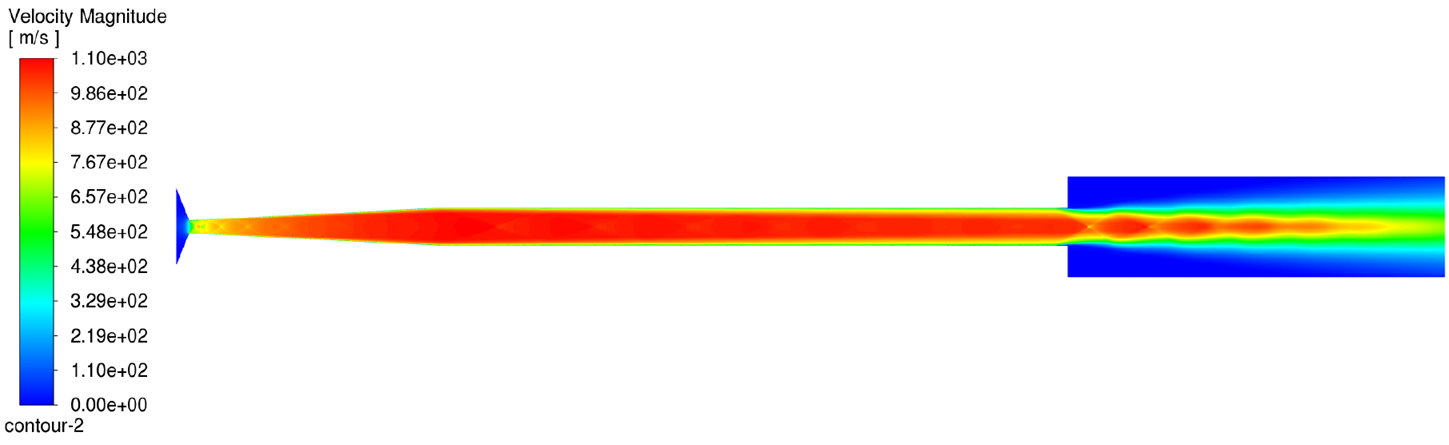
\includegraphics[width=1.0\linewidth]{imgs/velocipi.png}
	\caption[Resultados de la simulación del perfil de velocidad del gas en la tobera $T_{2}$]{Resultados de la simulación del perfil de velocidad del gas en la tobera $T_{2}$ \cite{CerdaLobos2024}.}
	\label{fig:velocipi}
\end{figure}

Entre las conclusiones principales del estudio de Cerda et al. destacan 
las siguientes. La tobera de diámetro de garganta de 0{,}5~mm no resulta 
conveniente, pues el flujo de gas se sobreexpande y se desprende de las 
paredes de la sección divergente, impidiendo el desarrollo completo del 
flujo supersónico y reduciendo la energía cinética transferida a las 
partículas por debajo del umbral de deposición. En cuanto a la longitud 
de la sección divergente, se verificó que a mayor longitud, mayor es la 
velocidad alcanzada por las partículas y, en consecuencia, mayor la 
eficiencia de deposición. 

\begin{figure}[h!]
	\centering
	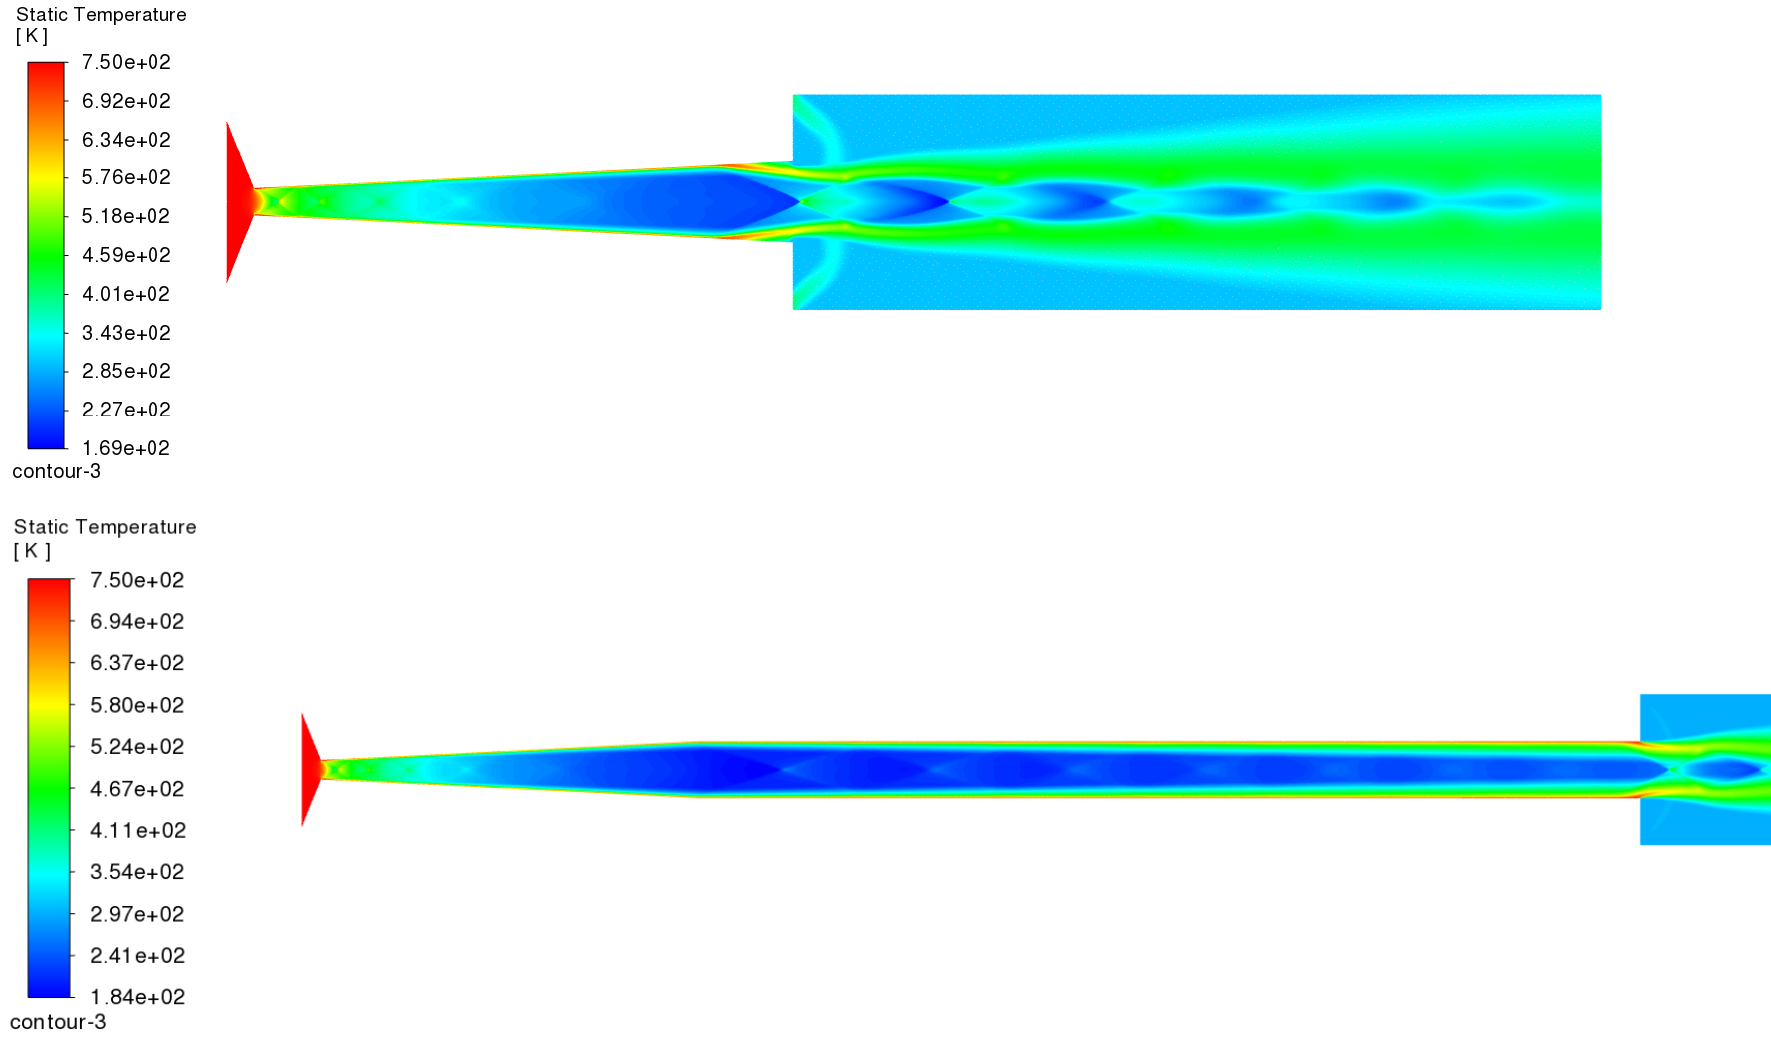
\includegraphics[width=1.0\linewidth]{imgs/tobtemps.png}
	\caption[Simulación para la temperatura del gas en toberas $T_{1}$ y $T_{2}$]{Simulación para la temperatura del gas en toberas $T_{1}$ y $T_{2}$ \cite{CerdaLobos2024}.}
	\label{fig:temp_gas}
\end{figure}

Finalmente, el análisis de mezclas N$_2$-He mostró aumentos significativos 
en la velocidad del gas y en la eficiencia de deposición, aunque los 
autores concluyen que, considerando únicamente los costos de gas y 
material, la configuración más conveniente es la tobera 
convergente-divergente-barril de garganta de 1{,}5~mm y longitud total 
de 70~mm (20~mm de sección divergente y 50~mm de sección barril) 
operando exclusivamente con nitrógeno.

En la Figura~\ref{fig:temp_gas} se presentan los perfiles de temperatura del
gas a lo largo del eje de la tobera obtenidos de la simulación. Se observa que la temperatura en regiones cercanas a la salida de las toberas difícilmente alcanza los 570 K (296° C). Estos
resultados confirman que el proceso es nominalmente
compatible protección de silicona a implementar en la máquina, validando el diseño del sistema de
protección descrito en la sección 3.1.3.



Ambas toberas serán evaluadas experimentalmente mediante una trayectoria
rectilínea de referencia, y la selección de la tobera de trabajo se realizará
de manera cualitativa en función de la facilidad de deposición: se preferirá
aquella que logre adherencia a menor velocidad crítica para igual flujo másico.
En caso de que la diferencia no sea apreciable, la selección se realizará
mediante análisis comparativo del perfil de depósito obtenido.

\subsection{Caracterización del perfil de deposición}

Una vez establecidas las condiciones operativas del sistema --- temperatura de
estancamiento $T_0$ y presión de estancamiento $p_0$ fijadas en los valores
máximos alcanzables por el equipo --- se realizan experimentos de variación
paramétrica para estudiar la influencia de las variables de trayectoria sobre
el perfil de depósito. Los parámetros estudiados son la velocidad de avance
$v_f$, el ángulo de deposición $\theta$ y la distancia de standoff $d_s$,
variados de manera individual manteniendo los restantes en sus valores de
referencia.

Cada condición experimental consiste en una pasada rectilínea simple sobre el
sustrato de aluminio. El perfil transversal del cordón resultante se caracteriza
mediante perfilometría óptica confocal (Keyence VK-5000), obteniéndose para
cada condición las siguientes variables geométricas de interés:

\begin{itemize}
	\item Ancho del cordón $w$ [mm]
	\item Altura máxima del cordón $h$ [mm]
	\item Área de la sección transversal $A_c$ [mm$^2$]
	\item Factor de forma $h/w$, indicador de la convexidad del perfil
\end{itemize}

Los datos de perfilometría se ajustan en primera instancia mediante mínimos
cuadrados a una función Gaussiana de la forma:

\begin{equation}
	h(y) = h_0 \exp\left(-\frac{y^2}{2\sigma^2}\right)
	\label{eq:gaussiana}
\end{equation}

donde $h_0$ es la altura máxima del cordón, $y$ es la coordenada transversal
respecto al eje de deposición y $\sigma$ es la desviación estándar del perfil,
relacionada con el ancho del cordón mediante $w = 2\sqrt{2\ln 2}\,\sigma
\approx 2{,}355\,\sigma$. Sin embargo, la distribución Gaussiana constituye
una aproximación que no siempre describe adecuadamente el perfil real: en
depósitos de aleaciones de titanio obtenidos por CS, se ha reportado que el
perfil puede presentar hombros pronunciados o una forma más plana en la zona
central, alejándose del decaimiento Gaussiano puro~\cite{Vanerio2021}. Por
esta razón, la calidad del ajuste Gaussiano se evaluará mediante el coeficiente
de determinación $R^2$, y en caso de ajuste insuficiente se explorarán
funciones alternativas, como la super-Gaussiana generalizada:

\begin{equation}
	h(y) = h_0 \exp\left(-\left(\frac{y^2}{2\sigma^2}\right)^n\right)
	\label{eq:supergaussiana}
\end{equation}

donde el exponente $n > 1$ controla la planicidad del perfil central y la
abruptitud de los flancos.

Complementariamente, se realizan cortes transversales de los cordones
depositados, seguidos de embutido metalográfico y pulido, para su observación
en microscopio óptico y/o electrónico de barrido. Esta preparación permite
evaluar la porosidad interna del depósito, la calidad de la interfaz
titanio/aluminio, la porosidad, la morfología de deformación de las partículas
individuales y la distribución de óxidos interpartícula, características
que no son accesibles mediante perfilometría superficial y que son
determinantes para la integridad del depósito~\cite{Huang2020, Yin2022review}.

Cabe señalar que no existe a priori un perfil de deposición óptimo universal, puesto que 
los criterios de evaluación relevantes son en parte contrapuestos. Un perfil de menor 
deposición presenta menor ancho y altura de cordón, lo que se traduce en mayor resolución 
geométrica y menor convexidad superficial, facilitando la compensación de pared en etapas 
posteriores. Sin embargo, este perfil reduce la tasa de fabricación. Un perfil de mayor 
deposición presenta el comportamiento inverso: mayor tasa de fabricación a expensas de 
menor resolución y mayor requerimiento de compensación. La selección del perfil de trabajo 
constituye por tanto una decisión de compromiso, condicionada por los objetivos específicos 
de cada geometría a fabricar.

El perfil observado en la Figura 3.14 no debe interpretarse, en forma directa, como una referencia para el diseño del \textit{toolpath} o la resolución de deposición, ya que, más allá de las condiciones específicas consideradas en la simulación, dicho resultado corresponde a un caso estático. En este contexto, la ausencia de desplazamiento relativo entre la tobera y el sustrato implica un tiempo de interacción continuo en un mismo punto, lo que conduce a una sobreestimación de la altura de depósito respecto a condiciones reales de proceso.

En un escenario dinámico, el desplazamiento de la tobera introduce tiempos de exposición finitos y espacialmente distribuidos sobre el sustrato, por lo que se espera una reducción significativa del espesor local del depósito. Adicionalmente, esta reducción no sigue necesariamente una dependencia lineal con la velocidad de la herramienta, debido a la naturaleza no lineal de la eficiencia de deposición, la superposición de impactos y los fenómenos de consolidación progresiva característicos del proceso de CS.

Por otro lado, el diámetro efectivo del \textit{spot} depositado sí puede considerarse comparable con el diámetro de garganta reportado en la literatura, lo que sugiere que el ancho del perfil simulado en la Figura 3.14 (del orden de 2 mm) es representativo de la zona principal de deposición. No obstante, en la periferia del \textit{spot} se observa una disminución significativa de la tasa de deposición, asociada a una menor densidad de impacto y a condiciones angulares menos favorables.

Asimismo, debe considerarse que este diámetro nominal del \textit{spot}, si bien, va a ser directamente observable en los bordes de la primera capa, no definirá la resolución del proceso. Al implementarse la compnesacipón olbicua de pared, esta podría apuntar desde una zona más al interior del perfil lejos de las zonas con menor concentracion. De esta forma, el ancho de pared efectivo es menor al spot nominal, y la superficie disponible para la siguioente capa tambien queda limitada a un ancho menor al perfil nominal de deposicion. En este sentido, una capa homogénea podría construirse a partir de aproximadamente 0.4 mm desde el centro del perfil mostrado en la Figura 3.14, concentrando la deposición en la región de mayor intensidad del \textit{spot}. Sería relevante entonces el estudio del perfil depositado en nuevas capas, sobretodo en torno al borde, y su comparación con el perfil en la primera capa.


\subsection{Estrategia de deposición planar}

El problema central en la fabricación por CS es que una pasada simple 
produce un cordón con perfil transversal convexo. Al superponer pasadas 
adyacentes o capas sucesivas sin compensación, el material se acumula de 
forma no uniforme, lo que genera una superficie irregular que se propaga y 
amplifica con cada capa depositada, así como una degradación progresiva de 
la definición de borde en las paredes de la pieza. En esta investigación se aplicará la \textbf{estrategia de teselación triangular} descrita en Wu et. al.

Para contrarrestar la pérdida de borde en las paredes, Chepillo et 
al.~\cite{Chepillo2024} y Wu et al.~\cite{WU2025642} definen la \textbf{deposición oblicua}, que consiste en ejecutar pistas 
de corrección sobre los trazos principales inclinando la pieza en el eje 
$A$, de modo de exponer el borde del cordón y depositarlo de manera 
efectiva. Esta técnica es la que gobierna la resolución de detalles 
puntuales y la conformación de estructuras de pared delgada.

Para sectores cuyo ancho supere el perfil de deposición individual, el 
volumen se genera mediante \textbf{solapamiento} de pistas interiores, de 
modo que la superposición de los perfiles aproxime una superficie plana. En 
caso de que el solapamiento induzca una ondulación residual que dificulte 
la deposición de capas sucesivas, esta puede atenuarse mediante pistas 
inter-trazo perpendiculares intercaladas entre los trazos de relleno, hasta 
alcanzar una planitud aceptable.

Para describir las trayectorias involucradas en la construcción de una 
pieza, se adoptará la nomenclatura propia de la impresión FDM, 
distinguiendo entre \textbf{pistas externas} (\textit{walls}), que definen 
la geometría superficial de la pieza con la tobera en orientación normal a 
la superficie, y \textbf{pistas interiores} o de \textbf{relleno} 
(\textit{infill}), que generan el volumen interior mediante solapamiento de 
cordones adyacentes. Adicionalmente, se definen \textbf{pistas de 
	corrección}, aplicadas con la tobera en orientación oblicua para compensar 
la pérdida de borde en las paredes, y \textbf{pistas inter-trazo}, 
intercaladas entre las pistas de relleno para atenuar la ondulación 
superficial residual. 

Para la fabricación de las piezas se adoptará una estrategia de 
\textbf{rasterizado concéntrico} y \textbf{rasterizado paralelo bidireccional} según sea conveniente, ejecutando las pistas en el siguiente 
orden: pistas externas, pistas interiores de relleno, pistas inter-trazo y, 
finalmente, pistas de corrección oblicua. En la Figura \ref{fig:trazos} se observa la nomenclatura descrita, donde una sección rectangular es fabricada a través de una estrategia paralela bidireccional compensada finalmente por una deposición oblicua contínua.

\begin{figure}[h!]
	\centering
	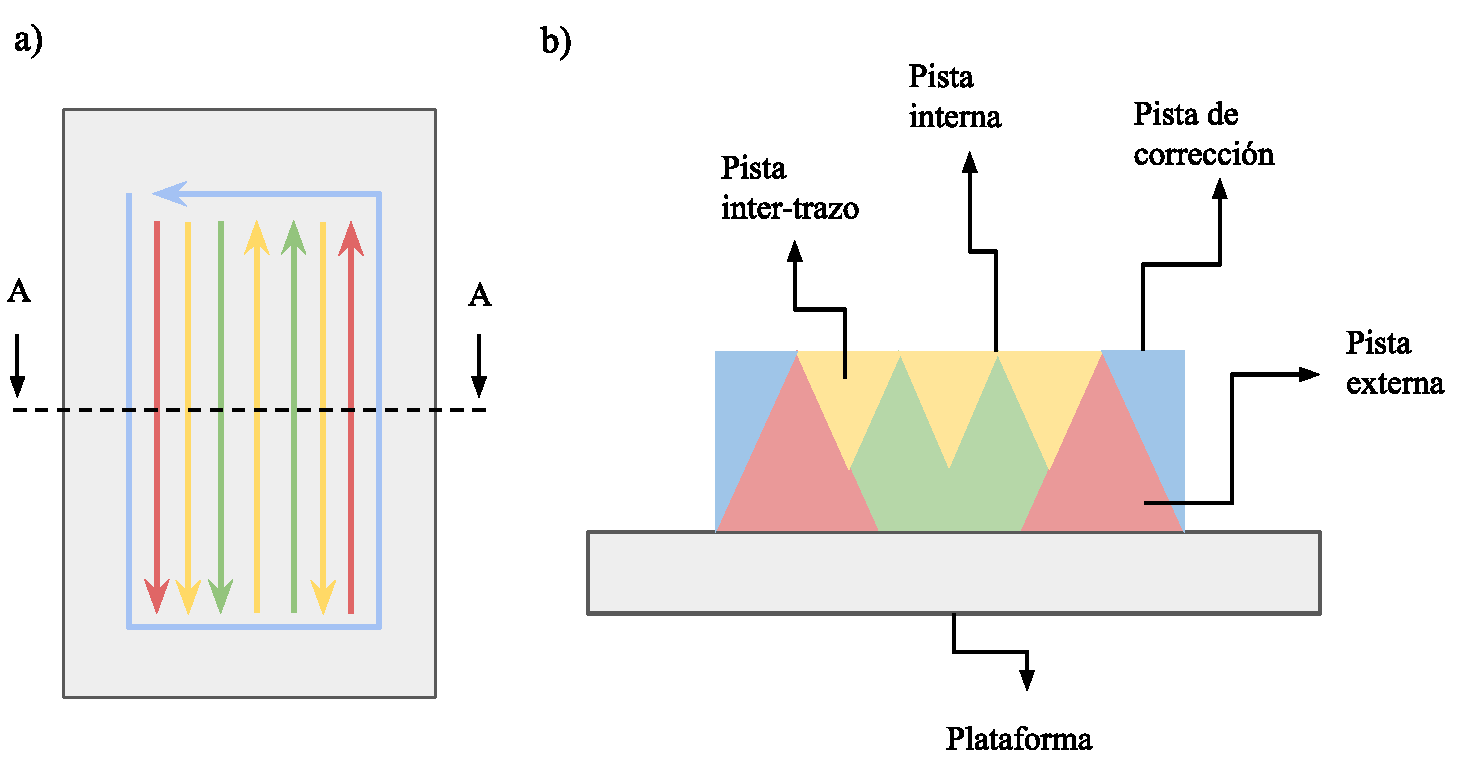
\includegraphics[width=0.9\linewidth]{imgs/transversal.pdf}
	\caption[Diagrama de teselación triangular en geometría rectangular y nomenclatura en la sección transversal]{Diagrama de teselación triangular en geometría rectangular y nomenclatura en la sección transversal, a) Vista superior de trayectorias para geometría rectangular y b) corte transversal.}
	\label{fig:trazos}
\end{figure}

Cabe notar que, a diferencia de la impresión FDM de polímeros, la 
fabricación de piezas metálicas implica requisitos de servicio potencialmente 
exigentes, por lo que la optimización de los parámetros operativos en cada 
sector de la pieza está directamente condicionada por las dependencias del 
perfil de deposición y el potencial de subsanación que pueda aportar un 
tratamiento térmico posterior. Por ejemplo, es probable que se quiera optimizar la precisión y el detalle en el exterior, mientras que en el interior se desea disminuir el tiempo de fabricación. Tal análisis queda fuera del alcance de este 
trabajo; en consecuencia, se operará con los mismos parámetros tanto para 
pistas externas como para pistas de relleno.

Para el estudio paramétrico de la compensación oblicua en pistas únicas, 
la calidad de la deposición se evalúa mediante dos criterios geométricos 
medidos por perfilometría confocal. El primero es el ángulo promedio de la 
pared depositada respecto a la perpendicular al sustrato, extraído del 
perfil transversal del depósito; un valor próximo a \ang{0} indica una 
pared de geometría vertical, como se muestra en la Figura \ref{fig:metris}. El segundo es la rugosidad de la superficie 
superior del cordón, caracterizada mediante el parámetro $R_a$, cuya 
minimización favorece la deposición uniforme de capas sucesivas. La 
estrategia, o combinación de estrategias, que produzca simultáneamente el 
menor ángulo de inclinación y el menor $R_a$ superficial será adoptada 
para la fabricación de las probetas y geometrías descritas en las etapas 
subsiguientes.

\begin{figure}[h!]
	\centering
	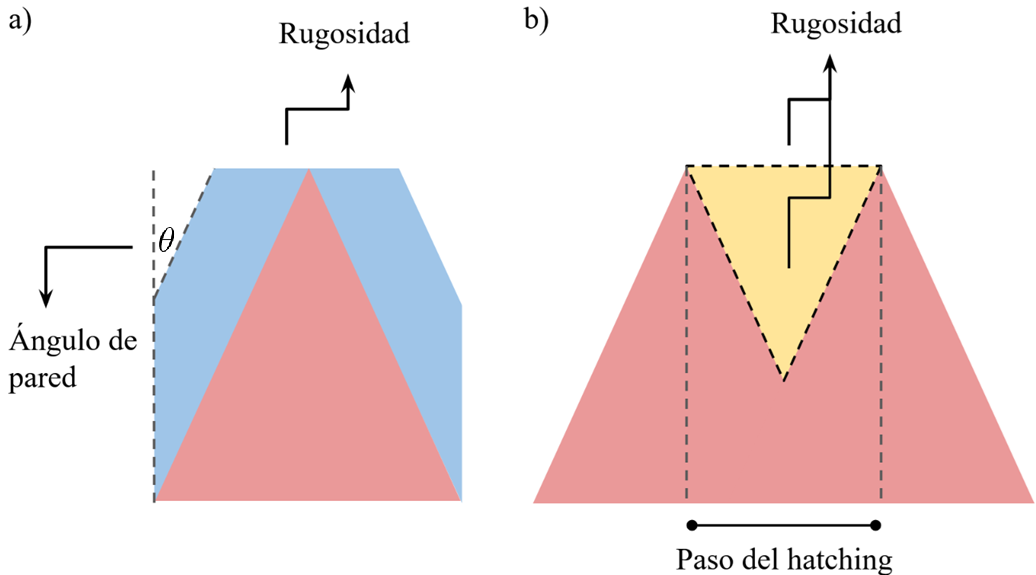
\includegraphics[width=0.8\linewidth]{imgs/metris.png}
	\caption[Diagrama para métricas de interés en experimentos planares]{Diagrama para métricas de interés en experimentos planares a) Pruebas de compensación oblicua y b) Pruebas de solapamiento.}
	\label{fig:metris}
\end{figure}

Del estudio de compensación oblicua se desprende también la posibilidad de 
explorar la generación de voladizos en condición de sobredeposición, en 
respuesta a los requerimientos expuestos en la Sección 3.2.6. En 
este caso, el criterio rector es igualmente la minimización de la rugosidad 
superficial de la pared resultante.

Para el estudio del solapamiento se evaluará la rugosidad superficial en 
función de la distancia entre pistas (\textit{hatch distance}), sin y 
con aplicar la corrección inter-trazo (Figura \ref{fig:metris}). Si bien el objetivo general 
es minimizar $R_a$, no se descarta que cierta rugosidad residual resulte 
beneficiosa para la adhesión de las capas sucesivas: Bruera et 
al.~\cite{Bruera2023adhesion} demuestran que, en cold spray, la relación 
entre rugosidad superficial y adhesión no es monótona, sino que existe un 
valor óptimo de rugosidad —del orden de $R_z \approx 34\,\mu\text{m}$ para 
el sistema Cu/AISI~304— a partir del cual la adhesión disminuye, y que 
dicho óptimo depende además de la dureza del sustrato. Dado que esta 
dependencia no ha sido caracterizada para el sistema Ti/Ti en condición de 
interfaz entre capas depositadas por CSAM, la determinación del criterio de 
optimización de $R_a$ requiere validación experimental en el presente 
trabajo.

Aun cuando determinadas configuraciones resulten exitosas en los estudios 
paramétricos, es previsible que emerjan limitaciones de distinta naturaleza. 
Existen, en primer lugar, restricciones inherentes al sistema: el volumen 
de trabajo disponible, los rangos de velocidad y aceleración alcanzables, y 
la resolución geométrica impuesta por el ancho del cordón depositado. Este 
último factor define un radio mínimo de curvatura por debajo del cual no es 
posible reproducir fielmente una trayectoria sin incurrir en solapamientos 
no deseados o en zonas sin cobertura.

Al trazar curvas, la velocidad tangencial del punto de deposición es mayor 
en el lado exterior del arco que en el interior, dado que ambos recorren el 
mismo ángulo en el mismo intervalo de tiempo pero a radios distintos. Esto 
produce una mayor acumulación de material hacia el interior de la curva y 
una potencial falta de cobertura en el exterior. En consecuencia, y en 
concordancia con los resultados de Vargas-Uscategui et 
al., se establece que las geometrías fabricadas no 
pueden presentar vértices de ángulo recto, sino que deben incorporar una 
curvatura mínima en los cambios de dirección del perímetro cuando este se 
recorre de forma continua.

Una segunda restricción deriva del carácter continuo de la deposición: 
deben minimizarse los depósitos indeseados en las zonas de transición entre 
pistas consecutivas. Las acciones contempladas para este fin incluyen el 
aumento puntual de la velocidad de travesía, la reducción del ángulo de 
incidencia y el alejamiento transitorio de la zona de deposición al término 
de cada pista.

Cabe señalar que ciertas limitaciones son propias de cada estrategia. La 
deposición con compensación oblicua, por ejemplo, introduce un efecto de 
sombra geométrica asociado al ángulo de inclinación de la boquilla y a la 
distancia de \textit{standoff}, lo que impone una separación mínima entre 
paredes paralelas fabricables sin interferencia mutua. La caracterización de 
estas restricciones delimita el espacio de geometrías alcanzables con el 
sistema y constituye el punto de partida para el análisis de deposición 
multicapa desarrollado en la etapa siguiente.

Se hace notar que los rangos operativos reportados por Chepillo et 
al.~\cite{Chepillo2024} no son directamente homologables al presente 
trabajo, dado que las simulaciones correspondientes se realizaron en 
condiciones ideales que no contemplan efectos inerciales de la máquina ni 
las perturbaciones asociadas a la dinámica real del sistema de 
posicionamiento., y se basan en el uso de cobre como material y aluminio como sustrato.

caracterizacion del perfil con perfilometro - standoff, velocidad - ancho, altura, convexidad.
metaloggrafica - porosidad, interfaz, 
solapamiento - distancia entre pistas - rugosidad
oblicuo - angulo de deposicion (velocidad, flujo, standoff) - angulo


\section{Planificación de experimentos multicapa}

\subsection{Estrategias multicapa}

La etapa de deposición multicapa constituye una extensión natural de los 
resultados obtenidos en la etapa anterior, en la que se establecieron 
estrategias exitosas para la generación de pistas simples. El primer paso 
consiste en replicar dichas estrategias de forma iterativa en la dirección 
$Z$ para la fabricación de una pared de altura creciente, midiendo ancho y 
altura al término de cada capa depositada.

No es evidente que las configuraciones óptimas para la primera capa sean 
transferibles al resto de la construcción. La geometría local de la 
superficie de deposición puede variar progresivamente por efecto de la 
acumulación de material y del endurecimiento por deformación acumulado en 
capas previas, alterando tanto el perfil del cordón como la compactación 
inter-capa. Por ello, se analiza la dependencia de la compensación 
requerida en función del número de capa, con el objeto de determinar si 
dicha compensación es constante, evoluciona linealmente o presenta un 
comportamiento más complejo que requiera corrección adaptativa por la pérdida de deposición (Figura \ref{fig:paredi}).

Posteriormente, se evalúa la fabricación de una pared alta en ángulo mediante capas con pared sobrecompensada en la deposición oblicua, lo que 
pone a prueba la capacidad de crecimiento de una sección en el plano $XY$ conforme se avanza en $Z$. 
Esta característica es necesaria para superar la restricción de sección 
transversal constante o decreciente que impone la deposición normal; sin 
ella, el espacio de geometrías producibles con el sistema quedaría 
significativamente reducido.

\begin{figure}[h!]
	\centering
	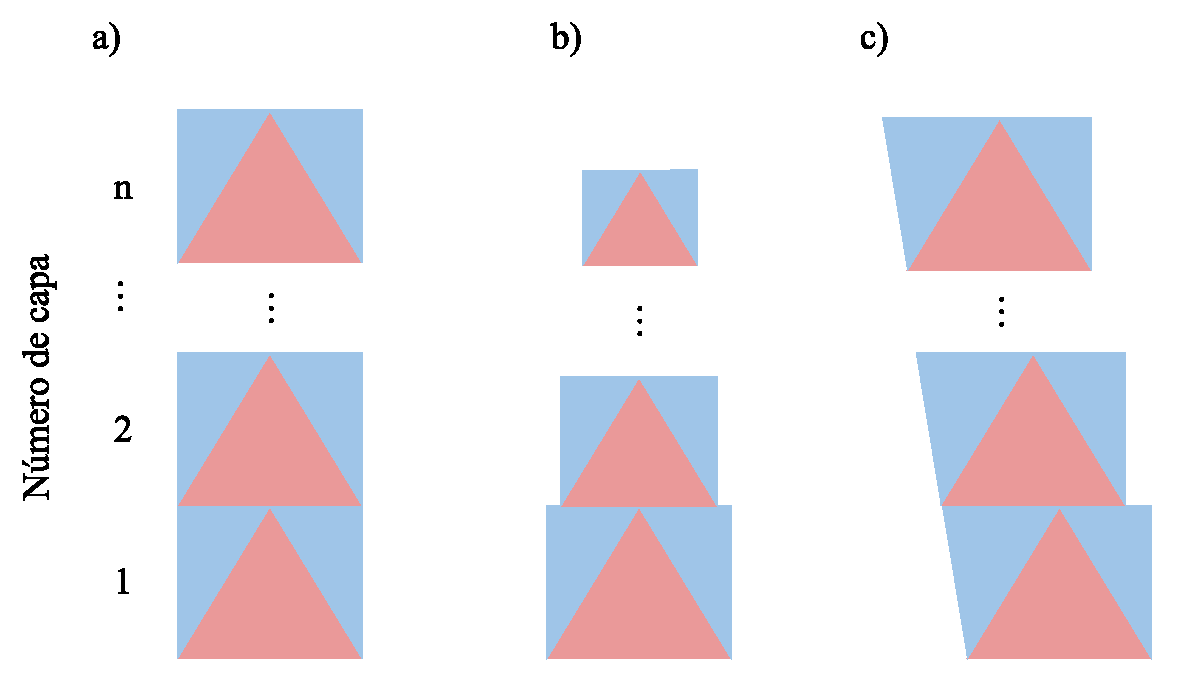
\includegraphics[width=0.8\linewidth]{imgs/pared.pdf}
	\caption[Diagrama de pruebas de pared alta multicapa]{Diagrama de pruebas de pared alta multicapa a) Caso ideal, b) Caso probable con pérdida de deposición y c) Prueba de pared oblicua.}
	\label{fig:paredi}
\end{figure}


Un aspecto crítico para la viabilidad de la fabricación aditiva multicapa 
es la adhesión entre capas sucesivas de material depositado por CS. A 
diferencia de la primera capa, donde la adhesión ocurre entre la partícula 
proyectada y el sustrato base, en las capas posteriores la deposición 
ocurre sobre material CS previamente consolidado. Esta condición es más 
exigente desde el punto de vista del mecanismo de enlace: la superficie 
del depósito previo presenta mayor resistencia a la deformación plástica 
como consecuencia del endurecimiento por deformación acumulado durante los 
impactos anteriores, lo que eleva efectivamente la velocidad crítica local 
requerida para la adhesión~\cite{Schmidt2006}. A esto se suma la 
posibilidad de oxidación superficial del titanio entre pasadas sucesivas, 
cuya capa de óxido nativo puede inhibir la formación de unión metálica 
directa entre partícula y sustrato~\cite{Huang2020}.

La evaluación cuantitativa de la adhesión inter-capa y su dependencia 
paramétrica —mediante análisis metalográfico de secciones transversales o 
caracterización del esfuerzo de corte inter-lámina— constituiría un 
criterio de aceptabilidad relevante para establecer interrelaciones entre 
velocidad de fabricación y resistencia mecánica inter-capa, así como para 
proyectar el efecto de un tratamiento térmico posterior sobre el conjunto 
de parámetros óptimos. No obstante, dicho análisis queda fuera del alcance 
de esta investigación, en la que se prioriza la constructibilidad y la 
precisión geométrica de las piezas por sobre su desempeño mecánico.

- conicidad
- angulo de voladizo
- metalografico 

\subsection{Geometrías 3D}

La validación del sistema como plataforma de fabricación aditiva se realiza mediante la 
fabricación de geometrías de complejidad creciente, evaluadas cualitativamente en términos 
de integridad estructural y con una \textbf{tolerancia dimensional de referencia de $\pm 2$ mm }
respecto a las dimensiones nominales de diseño, medida sobre las cotas principales de cada 
pieza. La progresión propuesta permite aislar las capacidades del sistema de forma 
incremental, de modo que cada nivel de complejidad introduce una nueva exigencia geométrica 
sobre los resultados de la etapa anterior.

El primer nivel corresponde a geometrías de extrusión plana con sección transversal 
constante, específicamente cajas rectangulares de borde redondeado y tubos cilíndricos de pared delgada sin 
tapa. Estas geometrías son simétricas y parametrizables de forma directa por lo que constituyen la validación más directa de la 
estrategia multicapa establecida en la subsección anterior. Su fabricación exitosa 
confirma la capacidad del sistema para mantener una sección transversal estable a lo 
largo de la dirección $Z$.

El segundo nivel introduce geometrías con variación de sección transversal en $Z$, 
específicamente conos y pirámides redondeadas. Estas piezas permiten evaluar 
la capacidad del sistema para fabricar geometrías con \textit{overhang} progresivo. La 
inclinación de cada capa respecto a la anterior introduce exigencias adicionales sobre 
la adhesión intercapa y sobre la planificación de trayectorias en el espacio de cinco ejes.

El tercer nivel corresponde a una pieza de referencia de geometría simple pero 
funcionalmente representativa de aplicaciones típicas del titanio, como un fitting 
tubular o una pieza de revolución con variación de diámetro. La elección de una pieza 
con referente en la industria permite contextualizar los resultados en términos de 
resolución geométrica y desviación dimensional alcanzables con el sistema establecido.

Finalmente, cabe mencionar nuevamente una restricción transversal a todas las geometrías: el sistema 
no dispone de un mecanismo para interrumpir el flujo de polvo durante el reposicionamiento 
de la herramienta entre segmentos de trayectoria. Por ello, el diseño del G-code debe 
privilegiar trayectorias continuas por capa, o bien contemplar zonas de deposición de 
sacrificio hacia las cuales se dirija el chorro durante los movimientos de transición. 
Esta restricción condiciona tanto la complejidad de las geometrías abordables como la 
estrategia de generación paramétrica de trayectorias implementada en Python.

\section{Medición de resultados}

\subsection{Caracterización mecánica de probetas}

Dada la complejidad de mecanizar probetas de tracción a partir de depósitos de
titanio obtenidos con el sistema implementado, la caracterización mecánica se
concentra en mediciones de \textbf{microdureza Vickers (HV)}. Esta decisión es coherente
con el enfoque principal de la investigación, que prioriza la demostración de
viabilidad del proceso CSAM con aleación de titanio a alta resolución geométrica
relativa, por sobre la caracterización exhaustiva de propiedades mecánicas bulk
del depósito. Las mediciones de microdureza se realizan siguiendo la norma ASTM E384 \textit{Standard Test Method for Microindentation Hardness of Materials}.

El Ti CP Grado~4 presenta, en estado bulk recocido, valores de dureza 
típicos en torno a \SI{200}{HV}, siendo el más resistente de los grados 
de titanio comercialmente puro debido a su mayor contenido de elementos 
intersticiales, particularmente oxígeno \cite{Leyens2003}. A diferencia 
de las aleaciones $\alpha$+$\beta$ como el Ti-6Al-4V, el Ti CP no 
responde al envejecimiento, por lo que el endurecimiento por tratamiento 
térmico quedaría limitado al recocido de alivio de tensiones. En depósitos 
obtenidos por proyección fría, es habitual que la microdureza 
\textit{as-deposited} supere la del material bulk recocido, como 
consecuencia de la deformación plástica severa acumulada durante el 
impacto de las partículas, efecto análogo al trabajo en frío 
\cite{Huang2020, Yin2022review}. 

En las probetas se evaluará el grado de endurecimiento por deformación inducido durante el proceso de CS, así como la homogeneidad mecánica del depósito. Los valores obtenidos permitirán inferir indirectamente el nivel de deformación plástica sufrido por las partículas de titanio durante el impacto, la calidad de consolidación interparticular y la posible presencia de gradientes microestructurales asociados a variaciones en las condiciones de deposición. Adicionalmente, el análisis de dureza contribuirá a identificar posibles efectos de oxidación, porosidad local o zonas con deficiente cohesión, parámetros que influirían directamente en el desempeño mecánico del recubrimiento.

Las probetas para este experimento consisten en secciones cuadradas con número de capas variable, con una longitud de arista de 20 mm, compuestas por todos los tipos de pista mencionados. Los datos se tomarán en los sectores indicados en la Figura \ref{fig:microdureza} y en ambas direcciones de construcción de la probeta. Se fabricarán muestras con varios números de capa para estudiar el cambio de dureza entre capas.

La norma ASTM E384 establece criterios geométricos para la realización de ensayos de microdureza Vickers, definiendo distancias mínimas entre indentaciones, entre estas y el borde de la muestra, así como requisitos relacionados con el espesor mínimo del material, los cuales dependen del tamaño de la huella de indentación caracterizada por la diagonal $d$.

Se utilizá una carga HV0.1 (100 gf), dado que corresponde a la condición más ampliamente reportada en la literatura para recubrimientos de titanio obtenidos por CS, permitiendo una adecuada resolución de las variaciones microestructurales del depósito. Para esta condición, la diagonal de indentación en titanio se encuentra típicamente en el rango de 30--40 $\mu$m, adoptándose de forma conservadora un valor representativo de $d = 40 \, \mu$m.

La norma indica que el espesor mínimo del material debe ser suficiente para evitar la influencia del sustrato sobre la huella de indentación, lo cual se expresa mediante el criterio:

\begin{equation}
	t \geq 10d
\end{equation}

Sustituyendo el valor adoptado de la diagonal, se obtiene:

\begin{equation}
	t \geq 10 \cdot 40 \, \mu m = 400 \, \mu m
\end{equation}

En consecuencia, se establece un espesor mínimo de probeta de 800 $\mu$m, lo que proporciona un margen de seguridad respecto al criterio normativo y permite asegurar la validez de las mediciones de microdureza bajo las condiciones experimentales definidas.

De forma adicional, la norma ASTM E384 establece que la distancia mínima entre indentaciones debe ser al menos tres veces la diagonal de la huella, mientras que la distancia de la indentación respecto al borde de la muestra debe ser como mínimo 2.5 veces dicha diagonal. Para el valor adoptado de $d = 40 \, \mu$m, estas distancias corresponden a:

\begin{equation}
	\text{Distancia mínima entre indentaciones} \geq 3d = 120 \, \mu m
\end{equation}

\begin{equation}
	\text{Distancia mínima al borde} \geq 2.5d = 100 \, \mu m
\end{equation}

Estos criterios aseguran que no exista interacción entre los campos de deformación plástica generados por indentaciones adyacentes ni influencia de superficies libres sobre la respuesta mecánica medida.

Debe notarse que el criterio de borde de la norma podría invalidar la toma de datos en las pistas de compensación oblicua, si es que estas tienen un ancho efectivo menor al designado.

\subsection{Caracterización de piezas tridimensionales}

La evaluación de cada pieza fabricada considera los siguientes indicadores:

medidas principales con pie de metro
cloud compare
cualificacion tactil



\subsection{Análisis de desempeño del proceso}

El desempeño global del proceso se evalúa mediante los siguientes indicadores operativos, calculados para cada condición experimental y para la fabricación de piezas:

\textbf{Eficiencia de deposición} $DE$: cuantifica la fracción de polvo suministrado que efectivamente se incorpora a la pieza.

\textbf{Tasa volumétrica de deposición} $\dot{V}_d$ [mm$^3$/s]: indica la productividad del proceso en términos de volumen de material consolidado por unidad de tiempo.

\textbf{Consumo específico de gas} $C_g$ [L/mm$^3$]: volumen de N$_2$ consumido por unidad de volumen depositado, calculado a partir del caudal másico de gas y la tasa volumétrica de deposición. Este indicador es relevante para proyectar la escalabilidad y costo operativo del proceso.

\section{Sumario}

\subsection{Resumen de experimentos de CSAM}

En los Cuadros \ref{tab:resumen_etapa2}, \ref{tab:resumen_etapa3} y \ref{tab:resumen_etapa4} se presenta el compilado de experimentos de CSAM a desarrollar en esta investigación, separados por etapa del flujo de trabajo.

% Requiere \usepackage{booktabs} y \usepackage{array} en el preámbulo

% ============================================================
% ETAPA 2
% ============================================================
\begin{table}[htbp]
	\centering
	\small
	\caption{Resumen de experimentos -- Etapa 2: Paredes simples.}
	\label{tab:resumen_etapa2}
	\renewcommand{\arraystretch}{1.5}
	\begin{tabular}{>{\bfseries}p{0.20\textwidth} p{0.22\textwidth} p{0.22\textwidth} p{0.26\textwidth}}
		\toprule
		Experimento & Objetivo & Variables / Respuesta & Resultado / Métrica \\
		\midrule
		Selección de tobera &
		Determinar la tobera de mayor eficiencia de deposición &
		Geometría de tobera (T1 vs.\ T2) / masa depositada &
		$DE$ \\
		\midrule
		Perfil de deposición &
		Caracterizar la geometría transversal del cordón individual en función de los parámetros operativos &
		$P_0$, $T_0$, $v_t$ / perfil transversal; sección metalográfica &
		Parámetros del ajuste gaussiano/super-gaussiano ($w$, $h$, $n$), $R^2$, porosidad \\
		\midrule
		Compensación por trayectoria oblicua &
		Determinar el conjunto de parámetros que minimiza la desviación angular de la pared respecto a la perpendicular &
		Ángulo de trayectoria, $v_t$, distancia entre pasadas / desviación angular de la pared &
		Ángulo óptimo, $v_t$ óptima, desviación angular residual \\
		\midrule
		Overhang &
		Caracterizar el ángulo máximo de voladizo alcanzable en una pared simple &
		Parámetros operativos, estrategia de trayectoria / ángulo de overhang &
		Ángulo máximo de overhang $\theta_{oh}$ \\
		\bottomrule
	\end{tabular}
\end{table}

% ============================================================
% ETAPA 3
% ============================================================
\begin{table}[htbp]
	\centering
	\small
	\caption{Resumen de experimentos -- Etapa 3: Multicapa.}
	\label{tab:resumen_etapa3}
	\renewcommand{\arraystretch}{1.5}
	\begin{tabular}{>{\bfseries}p{0.20\textwidth} p{0.22\textwidth} p{0.22\textwidth} p{0.26\textwidth}}
		\toprule
		Experimento & Objetivo & Variables / Respuesta & Resultado / Métrica \\
		\midrule
		Conicidad de pared multicapa &
		Cuantificar el ángulo de conicidad generado al apilar capas sucesivas de pared directamente sobre depósito previo &
		Número de capas $n$, parámetros operativos / perfil lateral de la pared &
		Ángulo de conicidad $\theta_c$ en función de $n$ \\
		\bottomrule
	\end{tabular}
\end{table}

% ============================================================
% ETAPA 4
% ============================================================
\begin{table}[htbp]
	\centering
	\small
	\caption{Resumen de experimentos -- Etapa 4: Piezas volumétricas.}
	\label{tab:resumen_etapa4}
	\renewcommand{\arraystretch}{1.5}
	\begin{tabular}{>{\bfseries}p{0.20\textwidth} p{0.22\textwidth} p{0.22\textwidth} p{0.26\textwidth}}
		\toprule
		Experimento & Objetivo & Variables / Respuesta & Resultado / Métrica \\
		\midrule
		Fidelidad dimensional &
		Evaluar la precisión geométrica de las piezas fabricadas respecto al diseño nominal &
		Estrategia de trayectoria, parámetros operativos / dimensiones principales &
		Error dimensional absoluto y relativo ($\Delta d$, $\Delta d / d_0$) \\
		\midrule
		Microdureza &
		Evaluar la homogeneidad de las propiedades mecánicas a lo largo de la dirección de construcción &
		Posición en dirección $Z$ / dureza Vickers &
		Perfil de $HV$ vs.\ posición, homogeneidad \\
		\bottomrule
	\end{tabular}
\end{table}

\subsection{Resumen de indicadores de evaluación de CSAM}

En el Cuadro~\ref{tab:indicadores} se resumen los indicadores utilizados para evaluar la viabilidad del proceso CSAM implementado como alternativa para la fabricación aditiva de componentes metálicos de alta resolución a partir de polvo de titanio.

\begin{table}[h]
	\centering
	\caption{Indicadores de evaluación del proceso CSAM implementado.}
	\label{tab:indicadores}
	\begin{tabular}{llll}
		\hline
		Indicador & Símbolo & Unidad & Método de medición \\
		\hline
		Desviación geométrica        & $\delta_g$      & mm / \%        & Calibre / escáner 3D \\
		Porosidad aparente           & $\phi$          & \%             & Análisis metalográfico \\
		Rugosidad superficial        & $R_a$           & $\mu$m         & Perfilometría \\
		Microdureza                  & HV              & —              & Vickers \\
		Eficiencia de deposición     & $DE$        & \%             & - \\
		Consumo específico de gas    & $C_g$           & L/mm$^3$       & Cálculo operativo \\
		Tasa volumétrica             & $\dot{V}_d$     & mm$^3$/s       & Perfilometría / geometría \\
		\hline
	\end{tabular}
\end{table}

\chapter{Resultados y discusión}

\section{Caracterización}
\input{conclu.tex}

% ver https://www.overleaf.com/learn/latex/Glossaries
% \input{glosario.tex} % opcional

%\nocite{*}
\bibliographystyle{ieeetr}
\bibliography{bibliografia}

% opcional ...
\begin{appendices}
\input{anexoA.tex}
\end{appendices}
\end{document}